\documentclass[a4paper,12pt,oneside]{book}

%-------------------------------Start of the Preable------------------------------------------------
\usepackage[english]{babel}
\usepackage{blindtext}
\usepackage{tabto}
\usepackage{enumerate}
%packagr for hyperlinks
\usepackage{hyperref}
\hypersetup{
    colorlinks=true,
    linkcolor=blue,
    filecolor=magenta,      
    urlcolor=cyan,
}

\urlstyle{same}
%use of package fancy header
\usepackage{fancyhdr}
\setlength\headheight{26pt}
\fancyhf{}
%\rhead{
\includegraphics[width=1cm]{logo}}
\lhead{\rightmark}
\rhead{
\includegraphics[width=1cm]{logo}}
\fancyfoot[RE, RO]{\thepage}
\fancyfoot[CE, CO]{\href{http://www.e-yantra.org}{www.e-yantra.org}}
\usepackage{graphicx}

\pagestyle{fancy}

%use of package for section title formatting
\usepackage{titlesec}
\titleformat{\chapter}
  {\Large\bfseries} % format
  {}                % label
  {0pt}             % sep
  {\huge}           % before-code
 
%use of package tcolorbox for colorful textbox
\usepackage[most]{tcolorbox}
\tcbset{colback=cyan!5!white,colframe=cyan!75!black,halign title = flush center}

\newtcolorbox{mybox}[1]{colback=cyan!5!white,
colframe=cyan!75!black,fonttitle=\bfseries,
title=\textbf{\Large{#1}}}

%use of package marginnote for notes in margin
\usepackage{marginnote}

%use of packgage watermark for pages
%\usepackage{draftwatermark}
%\SetWatermarkText{
\includegraphics{logo}}
\usepackage[scale=2,opacity=0.1,angle=0]{background}
\backgroundsetup{
contents={
\includegraphics{logo}}
}

%use of newcommand for keywords color
\usepackage{xcolor}
\newcommand{\keyword}[1]{\textcolor{red}{\textbf{#1}}}

%package for inserting pictures
\usepackage{graphicx}

%package for highlighting
\usepackage{color,soul}

%new command for table
\newcommand{\head}[1]{\textnormal{\textbf{#1}}}


%----------------------End of the Preamble---------------------------------------


\begin{document}

%---------------------Title Page------------------------------------------------
\begin{titlepage}
\raggedright
{\Large eYSIP2018\\[1cm]}
{\Huge\scshape Autotuning Of Controller For Drones\\[.1in]}
\vfill
\begin{flushright}
{\large{\textbf{\underline{Interns:}}}}\\
{\large Mahadev Mishal \\}
{\large Karthik Nayak \\}
{\large Amit Kumar \\}
\end{flushright}

\begin{flushright}
{\large{\textbf{\underline{Mentors:}}}}\\
{\large{Fayyaz Pocker\\}}
{\large{Vamshi Krishna\\}}
{\large{Simranjeet Singh\\}}
{\large Duration of Internship: $ 21/05/2018-06/07/2018 $ \\}
\end{flushright}

{\itshape 2018, e-Yantra Publication}
\end{titlepage}
%-------------------------------------------------------------------------------

\setcounter{tocdepth}{2}
\tableofcontents 
\cleardoublepage
\pagebreak
%\chapter[Project Tag]{Autotuning Of Controller For Drones}
\chapter{Autotuning Of Controller For Drones}

\section{Abstract}
Proportional-integral-derivative (PID) controllers are widely used in industrial systems despite the
significant developments of recent years in control theory and technology. They perform well for a wide class of processes. Also, they give robust performance for a wide range of operating conditions. Furthermore, they are easy to implement using analogue or digital hardware. In practical implementation of a controller and tuning its control parameter, there is a high
possibility that due to human intervention the process is not tuned to obtain optimum control. Also this method of hit and trial is not an efficient way. Hence we propose two methods of auto-tuning the PID and estimating the values of PID parameter for Pluto drone. The first method is based on Ziegler-Nichols approach and second method is iteration based Auto-Tuning.

\section{Completion status}
\begin{itemize}
  \item Implemented PID on AR-Drone model in Gazebo.
  \item Implemented position holding of Pluto drone using whycon marker by manual tuning
  \item Implemented position holding of Pluto drone using whycon marker by applying Ziegler-Nichols
  \item Implemented autotune on the AR-Drone model and tested it in Gazebo.
  \item Implemented autotune on Pluto drone using two different techniques.\\\\\
\end{itemize}

\section{Hardware parts}
\begin{itemize}
  \item \textbf{Pluto drone by Drona Aviation Pvt. Ltd.}
    \begin{itemize}
        \item \textbf{Introduction}\\
        A quadcopter, also called a quadrotor helicopter or quadrotor, is a multirotor helicopter that is lifted and propelled by four rotors. Quadcopters are classified as rotorcraft, as opposed to fixed-wing aircraft, because their lift is generated by a set of rotors (vertically oriented propellers).Quadcopters generally use two pairs of identical fixed pitched propellers; two clockwise (CW) and two counterclockwise (CCW). These use independent variation of the speed of each rotor to achieve control.In drones, each motor spins in the opposite direction of the adjacent motor as shown in Figure 1. This allows it to achieve vertical lift.
        \begin{center}
         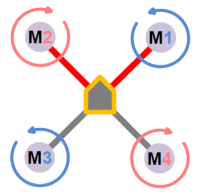
\includegraphics{quad_rotor.png}
        \end{center}
       \begin{center}
           figure 1
       \end{center}
        \item \textbf{Drone motion.}\\
        A drones’ thrust, roll, pitch and yaw is changed by manipulating the angular velocity of the motors. Following details how to move the drone by manipulating the angular velocity of the motors:
        \begin{enumerate}[I]
            \item \textbf{Thrust/Throttle}
             - In order to change the drones height, we can decrease or increase the velocity of all 4 motors. Reducing the velocity of all the motors lowers the drone height, while increasing the velocity increases the height of the drone with respect to the ground.
            \item\textbf{ Pitch}
            - By changing the motor speed of the front and back motors, we can move the drone forward and backward. Increasing the speed of the forward motors moves the drone back while increasing the speed of the back motors moves the drone backward.
            \item\textbf{ Roll} 
            - To move the drone left or right, we simply manipulate the left and right motors. By increasing the speed of the two left motors the drone bends to the right. By increasing the speed of the two right motors the drone bends to the left.
            \item\textbf{ Yaw} - By changing the speed of the alternate motors, the drone yaws to the left or right respectively
        \end{enumerate}
        \begin{center}
         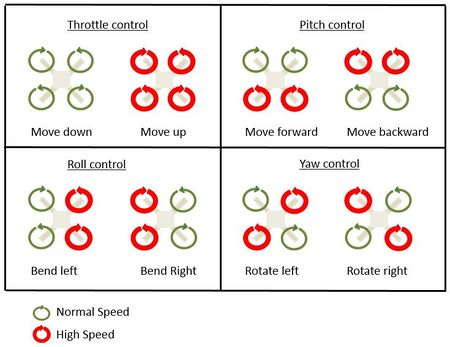
\includegraphics{roll.png}
        \end{center}
       \begin{center}
           Drone motion in 3D space
       \end{center}
        
    \end{itemize}
  \item \textbf{Wide angle camera}
  \item \textbf{Whycon marker\\}
  WhyCon is a vision-based localization system that can be used with low cost web cameras. It achieves millimeter precision with high performance. These markers consist of a dark Outer ring and a concentric white circle as shown in Figure
   \begin{center}
         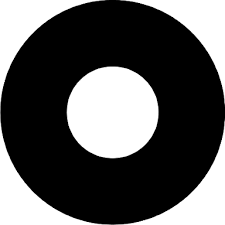
\includegraphics{whycon.png}
    \end{center}
    \begin{center}
          fig. Whycon marker
   \end{center}
  You can find more information about Whycon marker \href{https://github.com/eYSIP-2018/Autotuning-of-Controller-For-Drone/blob/master/Whycon_understanding.pdf}{here}
\end{itemize}

\section{Software used}
\begin{itemize}
  \item\textbf{ ROS \textit{indigo}}\\
  Robot Operating System (ROS) is a framework which provides tools and libraries to help software developers to create robot applications. The primary goal of ROS is to support code reuse in robotics research and development. Testing of robot code can be time-consuming and error-prone and sometimes physical robot might not be present. ROS provides a solution to this problem as it separates the hardware part and decision making (coding) part. Because of this separation, we can replace hardware part with a model in the simulator and test the behavior of decision-making part. It is open-source software. It also provides a simple way to record and play data.\\
  \item \textbf{Gazebo}\\
  Gazebo is a real world physics simulator. In this simulator, you can set up a world and simulate your robot moving around in this world. By installing  "\textbf{Desktop-Full}" version of ROS \textit{indigo} the simulator like \textbf{Gazebo, Rviz} also get installed.
  
  
 \item \textbf{Download link}
    \begin{itemize}
        \item Ubuntu 14.04 \\
        \href{http://releases.ubuntu.com/trusty/ubuntu-14.04.5-server-amd64.iso}{(64Bit)}/
        \href{http://releases.ubuntu.com/14.04/ubuntu-14.04.5-desktop-i386.iso}{(32 Bit)} 
        \item ROS \textit{indigo}\\
        \href{http://wiki.ros.org/indigo/Installation/Ubuntu}{download link}
    \end{itemize}
\end{itemize}

\section{ Arena Setup}
Below is the arena in which the Pluto drone will be made to fly.\\
\vspace{1em}
\begin{center}
    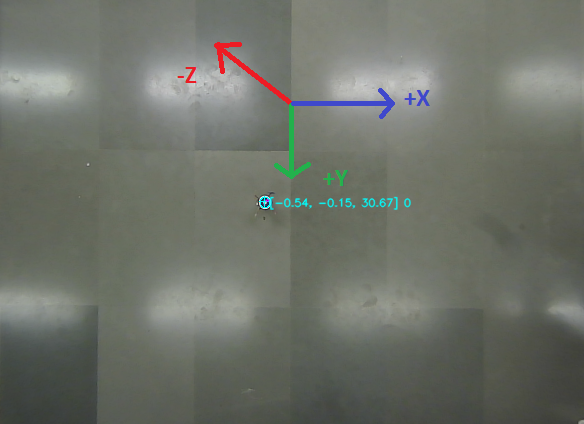
\includegraphics[width = 13cm , height= 10cm]{deck1.png}
\end{center}

\vspace{1em}

The x, y and z axes are as shown. As the z axis is w.r.t the overhead camera the +z axis is downwards.\\
Pitch axis of the drone is along the x-axis , roll axis is along y-axis and throttle is along z-axis.
To move in +x axis the pitch must be increased, the same must be decreased to move in -x axis.
To move in +y axis the roll must be increased, to move in -y axis  the same must be decreased
To move in +z axis the throttle must be decreased , to move it in -z axis it must be decreased.



\section{Software and Code}
%\href{http://www.github.com}{Github link} for the repository of code
\subsection{\textbf{Types of controller - }}
    \begin{itemize}
    \item \textbf{Proportional Controller (P Controller)}\\
             P controller is mostly used in first order processes with single energy storage to stabilize the
            unstable process. The main usage of the P controller is to decrease the steady state error of the system. As the proportional gain factor K increases, the steady state error of the system
            decreases. However, despite the reduction, P control can never manage to eliminate the steady
            state error of the system. As we increase the proportional gain, it provides smaller amplitude and phase margin, faster dynamics satisfying wider frequency band and larger sensitivity to the noise. We can use this controller only when our system is tolerable to a constant steady state error. In addition, it can be easily concluded that applying P controller decreases the rise time and after a certain value of reduction on the steady state error, increasing K only leads to overshoot of the system response. P control also causes oscillation if sufficiently aggressive in the presence of lags and/or dead time. The more lags (higher order), the more problem it leads. Plus, it directly amplifies process noise.
    \item \textbf{Proportional Derivative  Controller (PD Controller)}\\
            The aim of using P-D controller is to increase the stability of the system by improving control since it has an ability to predict the future error of the system response. In order to avoid effects of the sudden change in the value of the error signal, the derivative is taken from the output response of the system variable instead of the error signal. Therefore, D mode is designed to be proportional to the change of the output variable to prevent the sudden changes occurring in the control output resulting from sudden changes in the error signal. In addition D directly amplifies process noise therefore D-only control is not used. 
    \item \textbf{Proportional Integral Derivative (PID Controller)}\\
            P-I-D controller has the optimum control dynamics including zero steady state error, fast response (short rise time), no oscillations and higher stability. The necessity of using a derivative gain component in addition to the PI controller is to eliminate the overshoot and the oscillations occurring in the output response of the system.
    \end{itemize}

\subsection{P Controller}
A P controller consists of only a linear gain Kp. The output of such controller can be simply given as 
\begin{center}
\textbf{output  = Kp * error}
\end{center}   
 
\subsubsection{\textbf{Block diagram}}
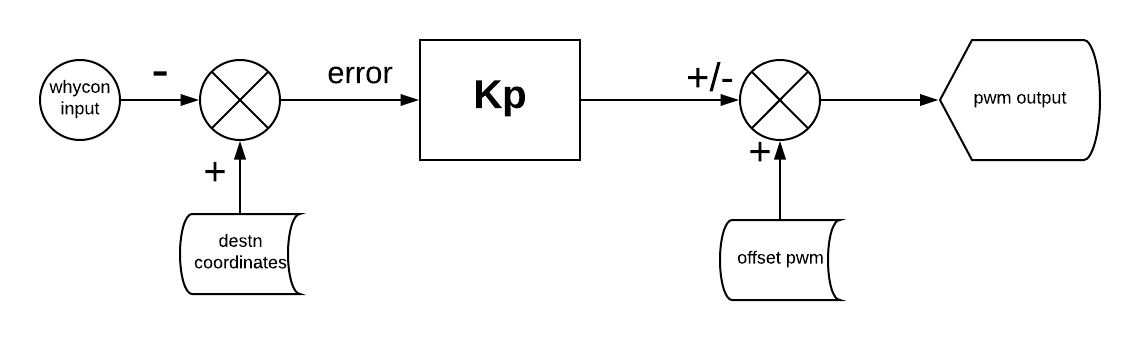
\includegraphics[width = 15cm , height= 5cm]{P.png}

The whycon input consists of x, y and z coordinates which gives the current location of the drone.\\
Suppose the destination is say, (x1, y1, z1), then the difference of coordinates i.e (x1-x) ,(y1-y), (z1-z) will be fed as an input to the P-controller.
The resultant product i.e Kp * error will be added or subtracted to the offset pwm as the need be to give the final output.\\


\href{https://github.com/eYSIP-2018/Autotuning-of-Controller-For-Drone/blob/karthik/P-controller.py}{Click here} to access the python program that implemented a P Controller on Pluto drone\\

\subsubsection{\textbf{Observations}}
It was observed that the drone never settled at its destination. Instead it oscillated about its destination.
The higher the value of Kp the more the amplitude of the oscillation and the drone would be out of the flying zone.\\

Below is a plot between error in x, y, and z coordinates and time. Clearly it is visible that the drone was not able to stabilise itself at the destination.\\ \\
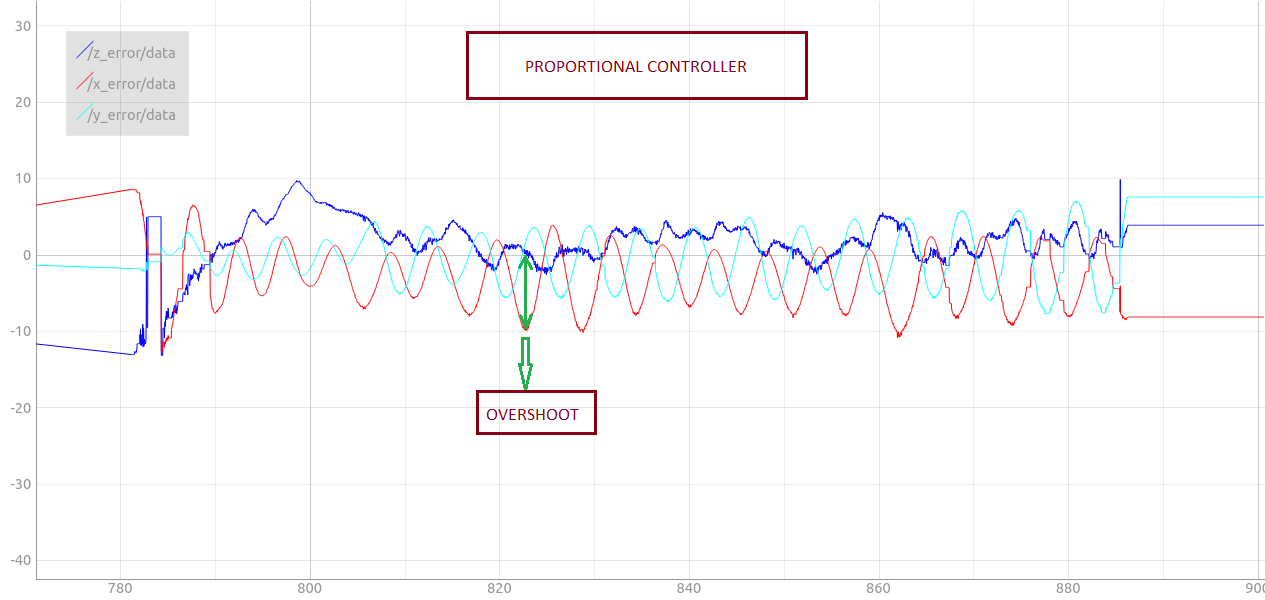
\includegraphics[width = 15cm , height= 10cm]{only-P(all).png}

Hence, it was concluded that a P-controller by itself wasn't able to stabilise the drone at a required point. \\

\subsection{PD Controller}
In the previous section we saw how the P-Controller wasn't successful in stabilising the drone at a given point. It was observed that there were oscillations instead. These oscillations can be damped by using a differential gain  along with the P-Controller. The system as a whole is said to be a PD Controller 

\subsubsection{\textbf{Block diagram}}
\begin{flushleft}
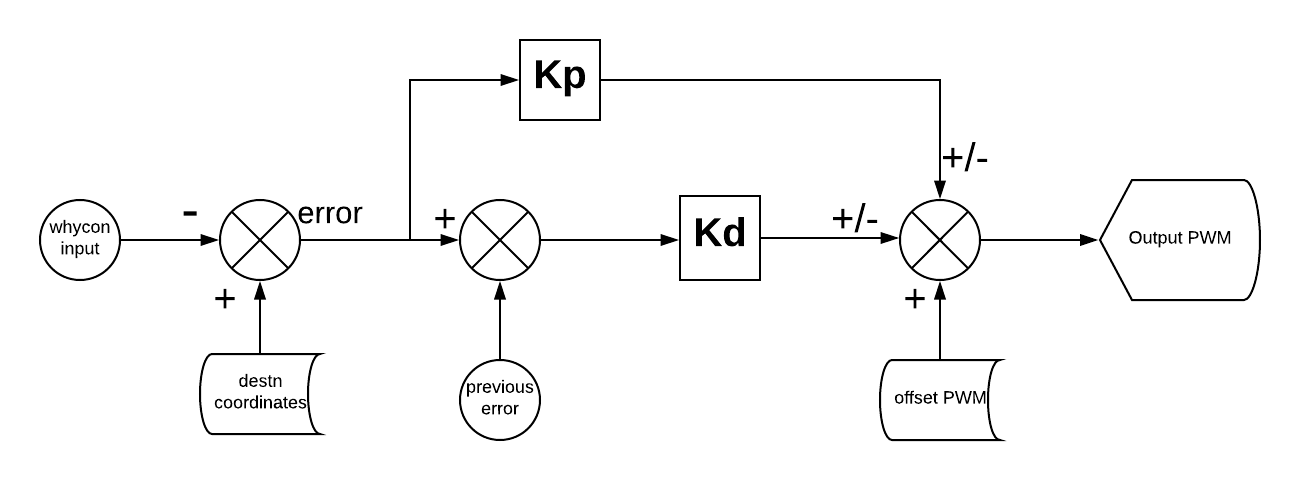
\includegraphics[width = 15cm , height= 10cm]{PD.png}
\end{flushleft}
The differential gain Kd is multiplied with the difference of error and previous error. Previous error is a variable that holds the last error generated by the controller output.\\
The controller output in this case is given as 
\begin{center}
\textbf{output  = Kp * error + Kd * (error - previous error)}  \\ 
\end{center} 
Note that Kd is calculated keeping the sampling time in consideration.\\
This output will be further  added or subtracted to the offset pwm as the need be to give the final output.\\ \\
\href{https://github.com/eYSIP-2018/Autotuning-of-Controller-For-Drone/blob/karthik/PD-controller.py}{Click here} to access the python program that implemented a PD Controller on Pluto drone\\

\subsubsection{\textbf{Observations}}
The results of this controller was no match to the P-controller.\\
The oscillations were damped with change in time.
Here is a plot of error and time for a PD controller implemented on the Pluto drone.
\begin{flushleft}
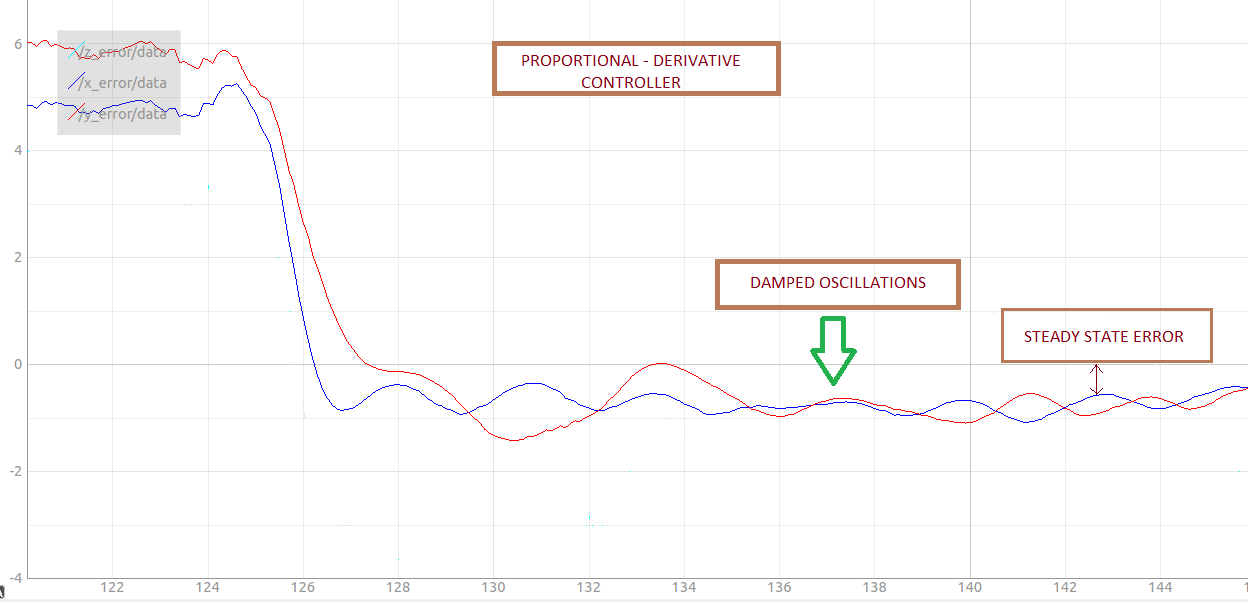
\includegraphics[width = 15cm , height= 10cm]{pd-controller.png}
\end{flushleft}
But, there was a hitch! \\
On having a closer look it was observed that though the drone could hover with respectable stability, it did not do so over the correct point, i.e the drone did not reach its destination instead it would hover at a point near to the destination.\\
This slight error is known as the steady state error.\\
Hence, it was concluded that a PD controller also by itself wasn't able to stabilise the drone at the correct destination.

\subsection{PID Controller}
In the previous section we saw how a PD controller was not quite enough.\\
In order to minimise the steady state error we introduce another gain called Ki ,the integral gain.\\
Such a system is said to be a PID Controller
\subsubsection{\textbf{Block diagram}}
\begin{flushleft}
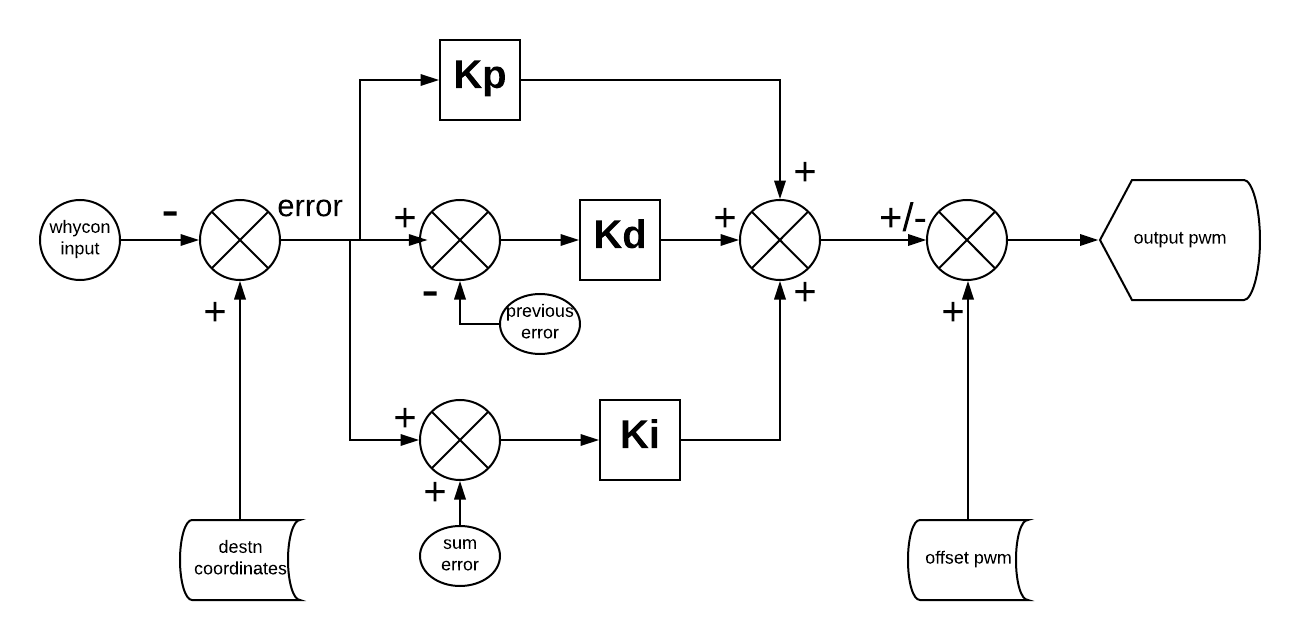
\includegraphics[width = 15cm , height= 10cm]{PID-controller.png}
\end{flushleft}
Here in we keep track of the error over time i.e sum up the errors over a specified sampling time.\\
\begin{center}
   \textbf{ Iterm = (Iterm + error) * Ki}
\end{center}
Further explanation regarding implementation of this Iterm is given in the code.\\
Note that Ki  is calculated keeping the sampling time in consideration.\\
This output will be further  added or subtracted to the offset pwm as the need be to give the final output.
\begin{center}
    \textbf{output = Kp*error + Iterm + Kd*(error - previous error)}
\end{center}
\href{https://github.com/eYSIP-2018/Autotuning-of-Controller-For-Drone/blob/karthik/PID-controller.py}{Click here} to access the python program that implemented a PID Controller on Pluto drone\\
\subsubsection{\textbf{Observations}}
The PID controller was successful in hovering the drone above the destination point with minimal error .\\
It overcome the steady state error which was noticeable in previous controllers.
Here is a plot of error and time for a PID controller implemented on the Pluto drone.
\begin{flushleft}
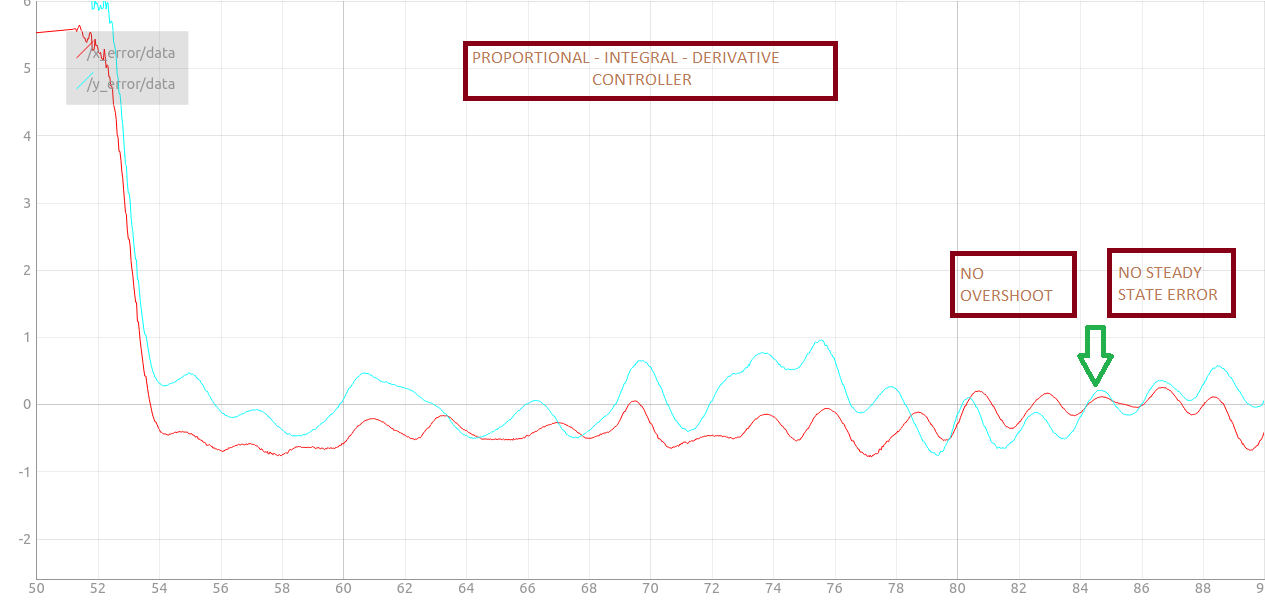
\includegraphics[width = 15cm , height= 10cm]{pid-1-no-z.png}
\end{flushleft}
 


\subsubsection{To sum it up}
\begin{flushleft}
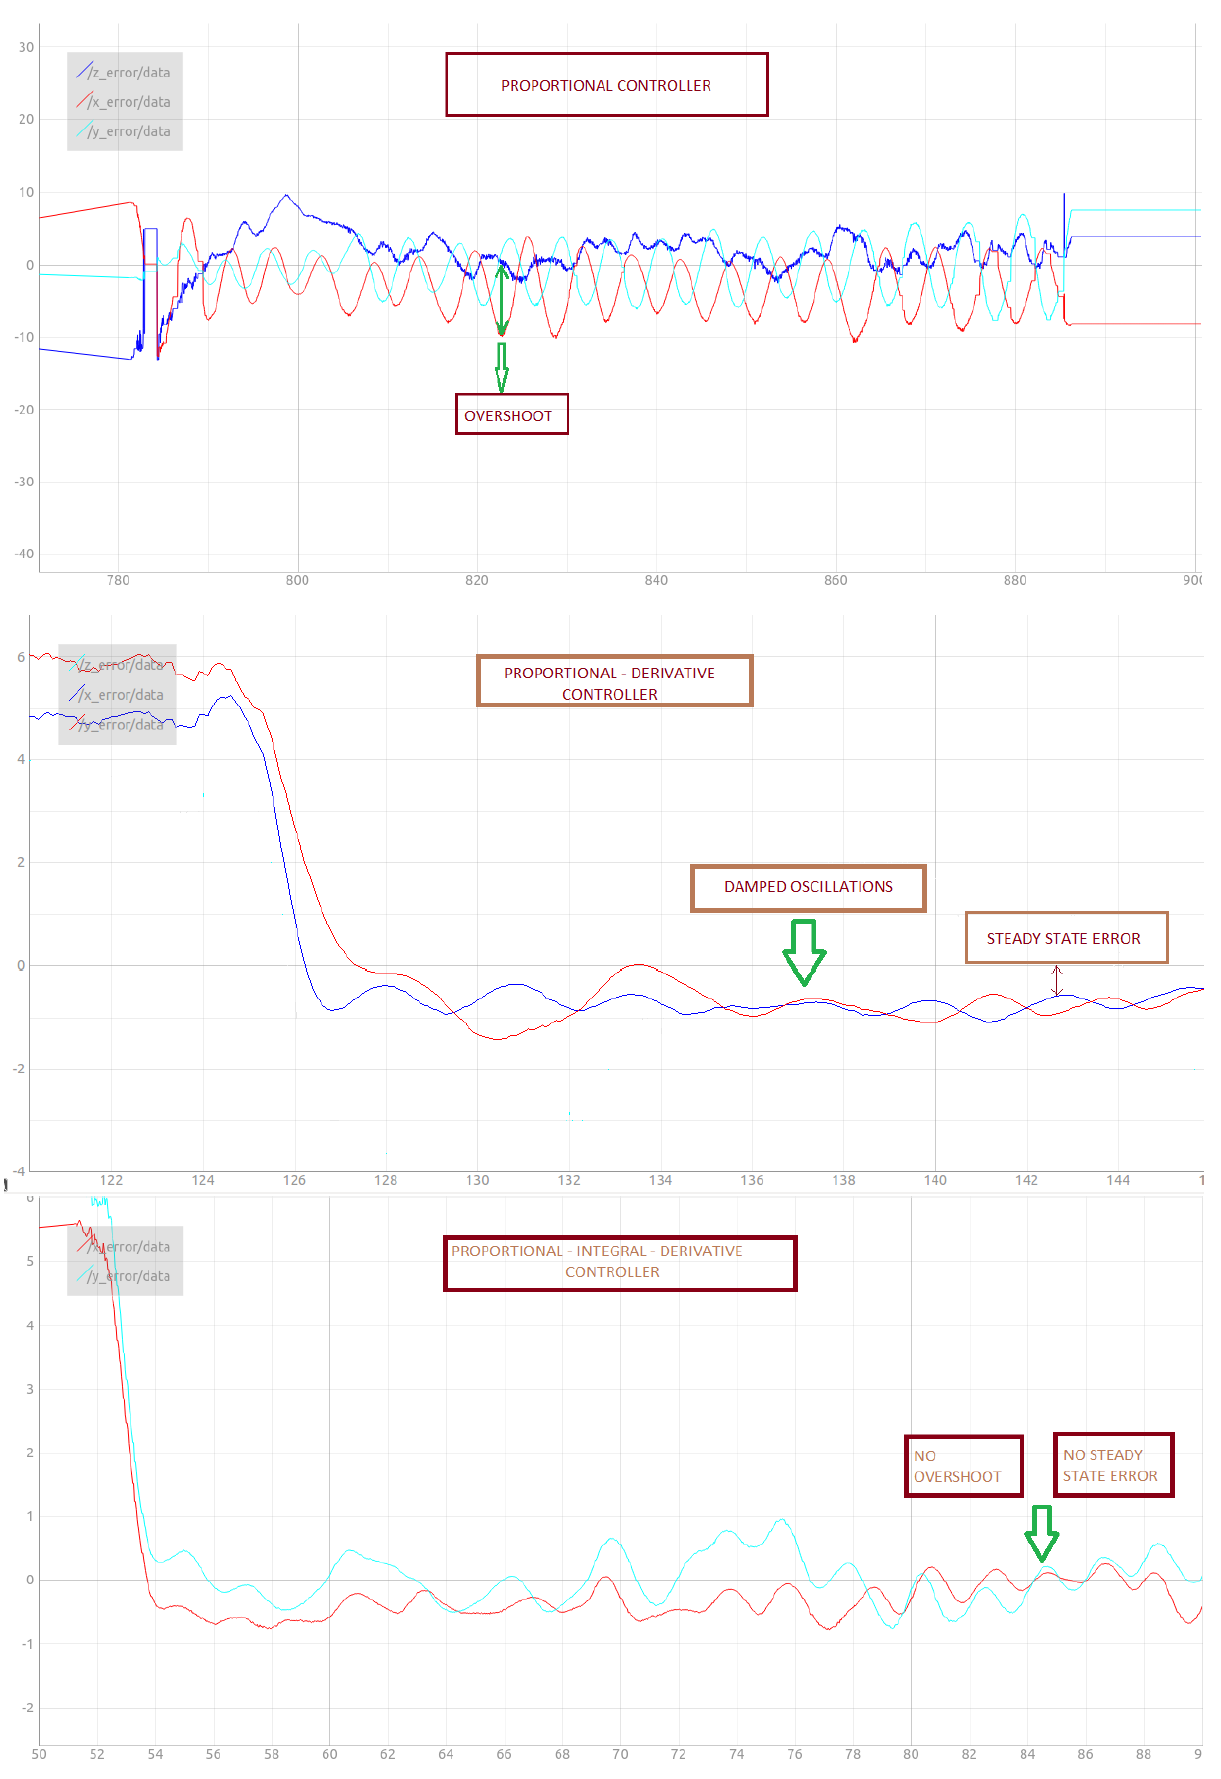
\includegraphics[width = 15cm , height= 20cm]{ALL_PID1.png}
\end{flushleft}

\subsection{Manual Tuning - A tedious job!}
The constants Kp, Ki and Kd need to be tuned to get the best response, however this job of tuning them manually is tedious.\\
Moreover if trial and error method is used to tune it , it may take longer time and may also compromise on efficiency.

\subsubsection{\textbf{The Solution}}
In order to reduce the human effort and time spent in tuning these parameters manually it is worth finding solutions that could somehow auto-tune these parameters.\\
In this project we propose two such methods.\\

\subsection{Auto-tuning of Controllers}
In this section we present two methods of auto-tuning.
\begin{enumerate}
    \item \textbf{Auto-tuning based on Ziegler-Nichols approach  }
    \item\textbf{Iteration based auto-tuning}
\end{enumerate}

\subsubsection{1. Auto-tuning based on Ziegler-Nichols approach}
In this method of auto-tuning we try to analyse the nature of what the controller is driving, then reverse-engineer to calculate tuning parameters from the output.\\
We do this by  changing the PID Output and then observe how the Input responds.

\subsubsection{Algorithm}
\begin{enumerate}
    \item Force the PID output to maximum.
    \item Wait for the input(hereon the drone's current location will be referenced as input), to cross above the setpoint(destination).
    \item Once the input is above the setpoint, force the PID output to minimum.
    \item Wait for the input to cross below the setpoint and then again force the PID output to maximum again.
    \item This constitutes an oscillation about the setpoint. Keep track of the time period of oscillations
    \item Determine Ultimate Gain ,Ku as
        \begin{center}
            \textbf{Ku = (4*d)/(pi*A)}
        \end{center}
        where,\\
        d --$>$ amplitude of PID output\\
        a --$>$ amplitude of oscillation about the setpoint
    \item The period of oscillation is known as Ultimate period \textbf{Tu}
    \item Use Ziegler-Nichols method to determine the values of Kp, Ki, Kd.
\end{enumerate}
More about Ziegler-Nichols approach in next section.!

\subsubsection{Ziegler - Nichols method of tuning PID constants}
The Ziegler–Nichols tuning method is one the methods to tune a PID controller. It was developed by John G. Ziegler and Nathaniel B. Nichols. Initially the integral gain, Ki and derivative gain, Kd, are set to zero. The proportional gain,Kp is then increased (from zero) until it reaches the ultimate gain Ku, at which the output of the control loop has stable and consistent oscillations.\\
This Ultimate gain Ku and Ultimate period Tu are eventually used to determine the Kp, Ki and Kd values.\\
The following table establishes the relation between the above mentioned parameters.\\


\begin{tabular}{|p{10em}|p{8em}|p{4em}|p{4em}|}\hline
		\textbf{Controller type} & \textbf{Kp} &\textbf{Ti} & \textbf{Td}\\\hline
		P  & 0.5 * Ku & $-$ & $-$\\\hline
			PI & 0.5 * Ku & Tu/1.25 & $-$\\\hline
PD & 0.8 * Ku & $-$ & Tu/8 \\\hline
Classic PID & 0.6 * Ku & Tu/2 & Tu/8\\\hline
	Pessen Integral rule & 0.7 * Ku & Tu/2.5 & 3Tu/20 \\\hline
Some overshoot & 0.33 * Ku & Tu/2 & Tu/3\\\hline
No overshoot & 0.2 * Ku & Tu/2 & Tu/3\\\hline

\end{tabular}
\vspace{1em}


Depending upon the need an appropriate controller type is selected and their corresponding equations can be used to compute the required parameters.\\
From the values of Ti, Td, and Kp it is possible to deduce the values of 
Ki and Kd as,
\begin{center}
    \textbf{Ki = Kp/Ti}\\
    \textbf{Kd = Kp * Td}
\end{center} 
\vspace{1em}
Once Kp, Ki, Kd are determined they can be just entered into the previously designed PID architecture.


\subsubsection{Simulation on AR-Drone in Gazebo}
The auto-tuning logic was applied to determine the Kp, Ki and Kd values of the PID controller that controlled the motion of the ARDrone.

\href{https://github.com/eYSIP-2018/Autotuning-of-Controller-For-Drone/blob/karthik/auto-ar.py}{Click here} to access the python program that simulated an auto-tuned PID Controller on AR drone in Gazebo\\

\subsubsection{Observations}
The auto-tuned values of Kp, Kd and Ki were properly tuned and the PID could bring about stable way point navigation of the drone.\\

Here are a couple of plots that were obtained during the simulation\\
\begin{flushleft}
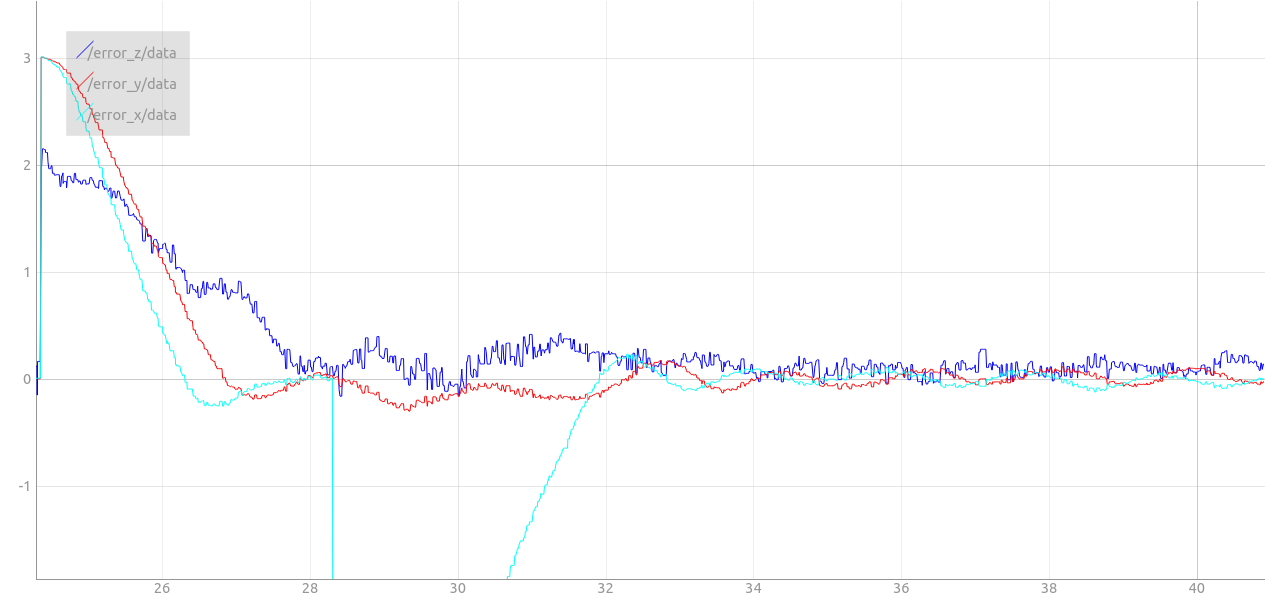
\includegraphics[width = 15cm , height= 8cm]{auto-tuning-ARDrone.png}

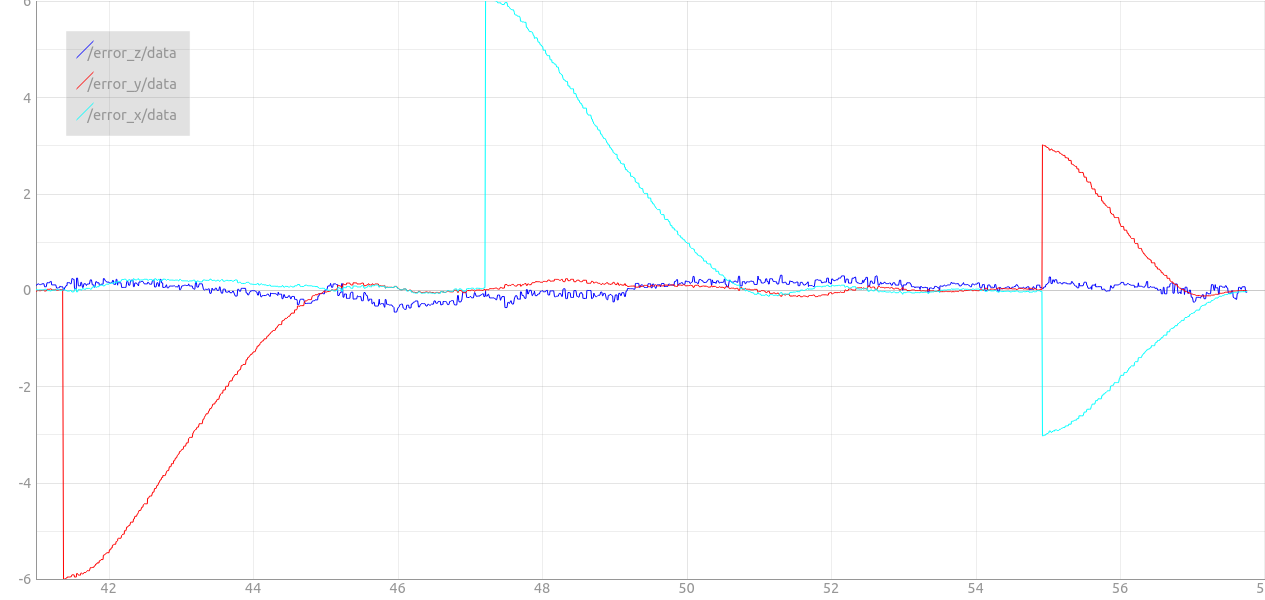
\includegraphics[width = 15cm , height= 10cm]{auto-tuning-ARDrone_2.png}

\end{flushleft}
After successful simulation of auto-tuning logic on AR-Drone in Gazebo, the same logic was applied for a Pluto drone.\\
The next section deals with the implementation of auto-tuning logic on Pluto Drone.

\subsubsection{Implementation on the Pluto drone}
The concept of auto-tuning based on Ziegler-Nichols was tested on the Pluto drone.\\
The drone was forced to oscillate on the z, x and y axis in order to determine the Ultimate gain, Ku and Ultimate period, Tu.

\href{https://github.com/eYSIP-2018/Autotuning-of-Controller-For-Drone/blob/6a7bdb9e7e259bd5313f333f7c46013b20c9bdca/auto-tuning-doc.py}{Click here} {to access the python program that implemented an auto-tuning of PID Controller of Pluto Drone} \\
The auto-tuning was performed on the drone for various types of PID as given in the previous table.

\subsubsection{Observations}
Auto-tuning performed by taking constant expressions from the previous table for classic PID, Pessen Integral rule, Some overshoot PID and No overshoot PID yielded good results.\\
Below are the plots of error vs time for each of the above mentioned cases.
 \subsubsection{Classic PID}
 \begin{flushleft}
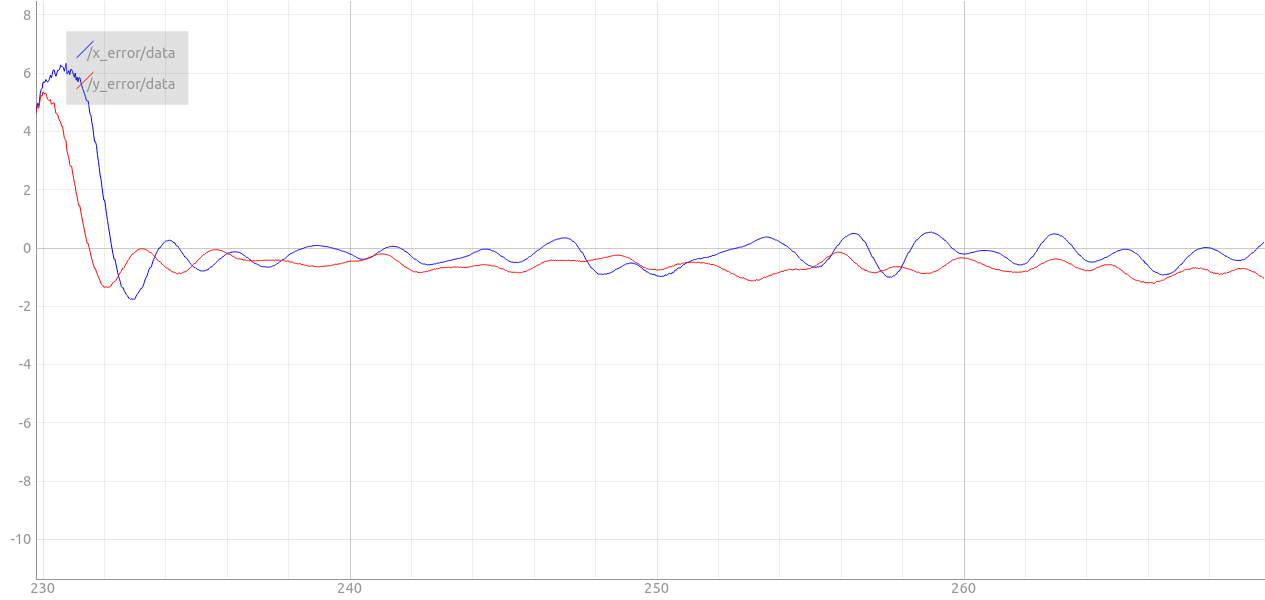
\includegraphics[width = 15cm , height= 8cm]{extra-1.png}
\end{flushleft}

\subsubsection{Pessen Integral rule}
\begin{flushleft}
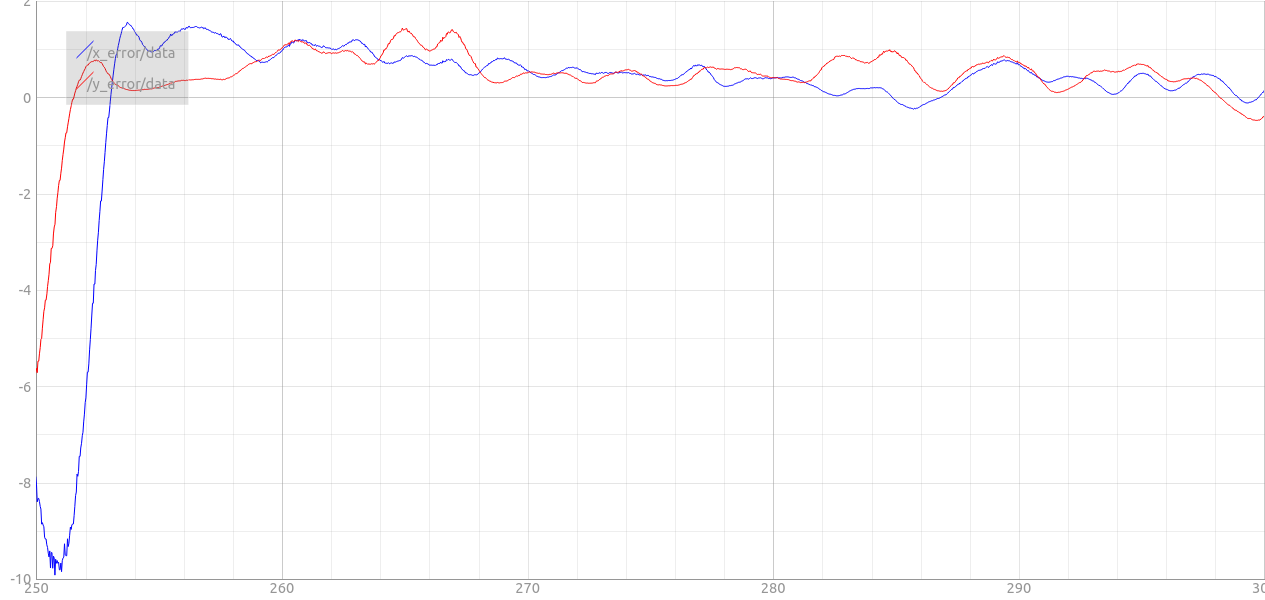
\includegraphics[width = 15cm , height= 8cm]{Pessen-rule.png}
\vspace{1em}
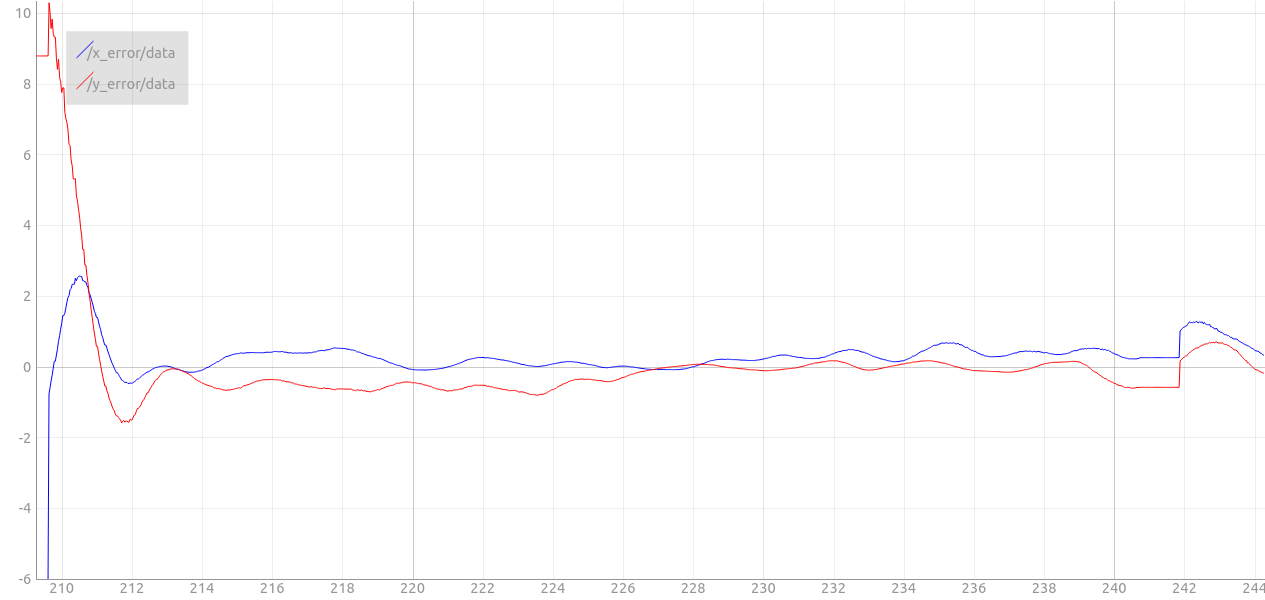
\includegraphics[width = 15cm , height= 8cm]{pessen-rule2.png}
\end{flushleft}

\subsubsection{Less Overshoot PID}
\begin{flushleft}
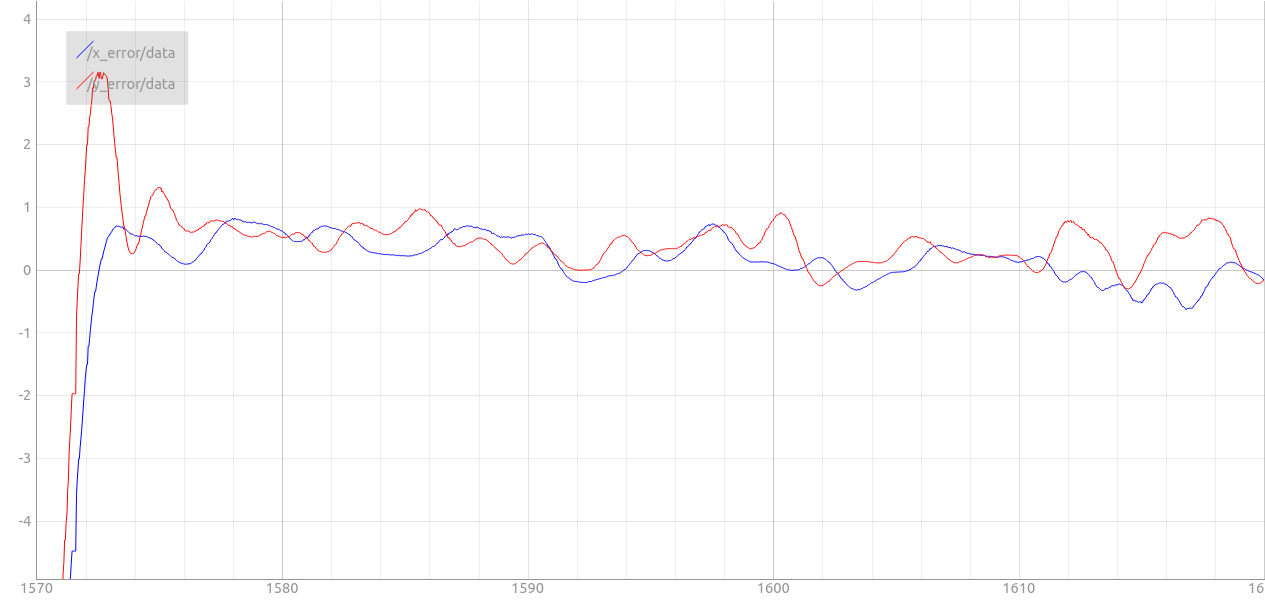
\includegraphics[width = 15cm , height= 8cm]{less-overshoot-pid.png}
In this, it is expected that there will some overshoot above the setpoint.
\end{flushleft}
 
 \subsubsection{No Overshoot PID}
\begin{flushleft}
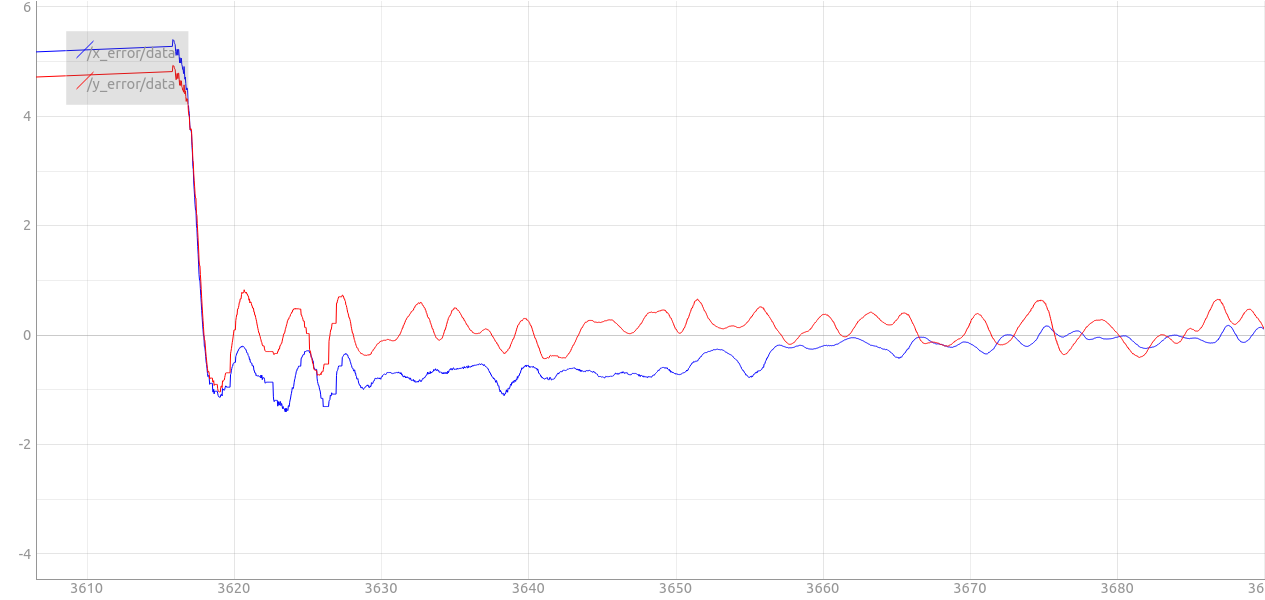
\includegraphics[width = 15cm , height= 8cm]{No-overshoot-pid.png}
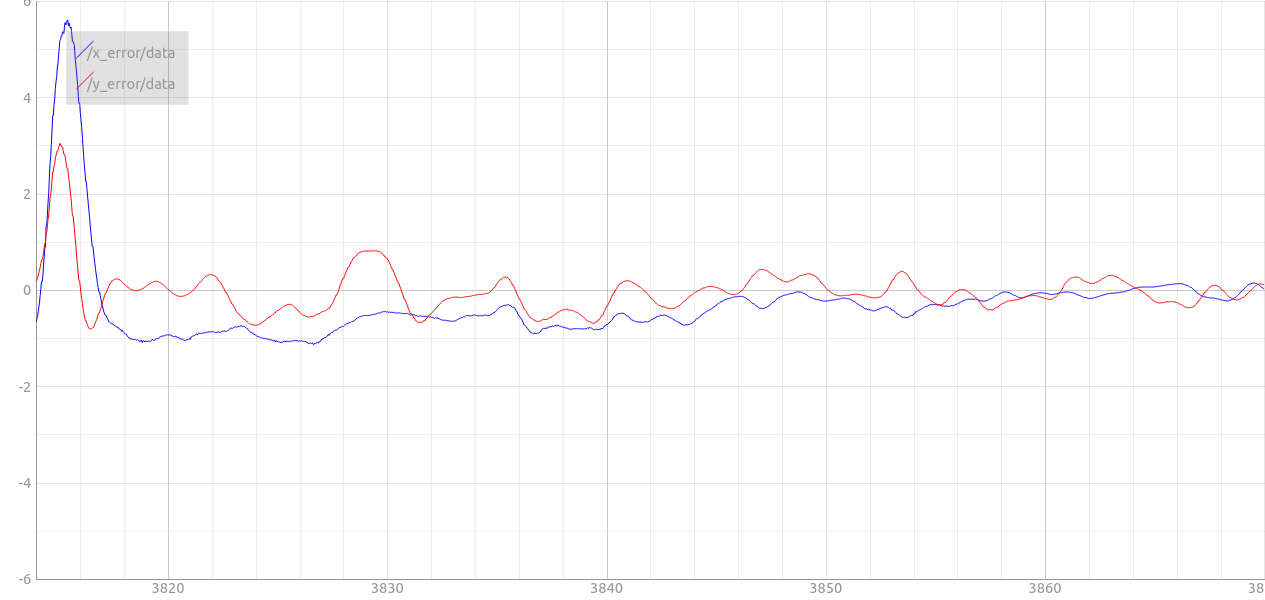
\includegraphics[width = 15cm , height= 8cm]{no-overshoot-pid2.png}
\end{flushleft}
In this, it is expected that there will not be any overshoot above the set point.
 
Depending upon the need and suitability any of the above types can be selected for use.

\subsubsection{Advantages}
\begin{itemize}
    \item The PID parameters could be found automatically and it is found to be consistent
    \item It was observed that the constants do not change over consistent period of time hence, we can only auto-tune it once and just use the obtained constants over and over again.
\end{itemize}

\subsubsection{Disadvantage}
\begin{itemize}
    \item The drone must be monitored while auto-tuning so that it doesn't go out of camera frame.
    ( watch the video in demo section for better understanding)
\end{itemize}

  
   
   
  
    














































\subsubsection{2. Iteration Based Auto - Tuning}

This method calculates optimum values of PID parameters for the controller by tuning during the flight. The user enters a range for the possible values of the parameters and the code continuously changes them based on the principles of control theory.

\subsubsection{Algorithm}
\begin{enumerate}
     
\item Set Kp, Ki and Kd of pitch and roll to minimum. 
\item Set Kp to maximum and Ki, Kd of altitude to minimum.
\item Increase Kp wrt rate of change of error for roll and pitch and decrease for altitude.
\item After the drone crosses a sphere of radius 1.8 units ten times, Kp is set constant.

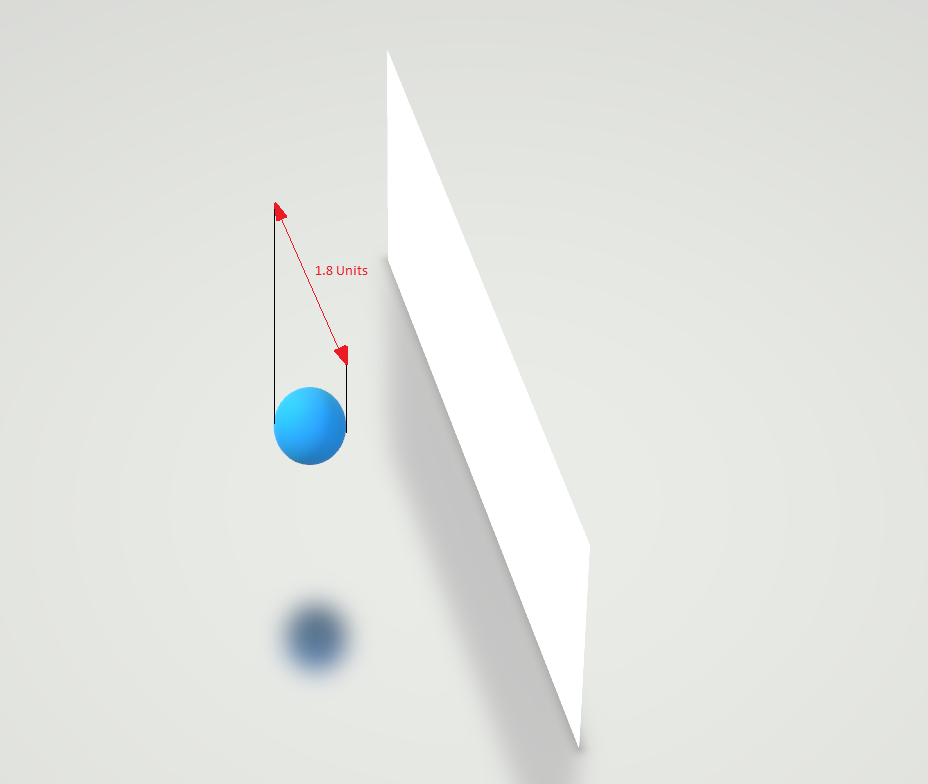
\includegraphics[width = 12cm , height= 6cm]{Capture.png}


\item Kd is increased again wrt rate of change of error till twice amplitude is less than 1 unit (for fifty cycles)

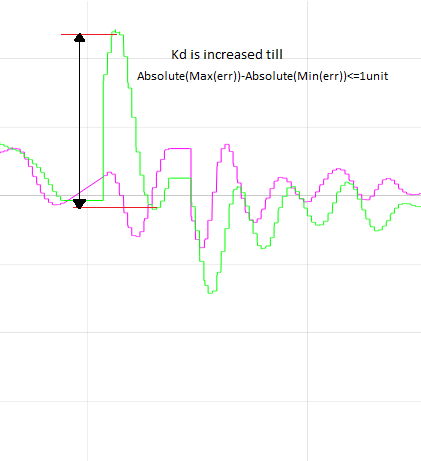
\includegraphics[width = 8cm , height= 5cm]{Autotune_iteration_1_e1.png}


\item Then Ki and Kd are changed till the drone maintains itself in a position of 0.8 units circle (for ten seconds)
\end{enumerate}


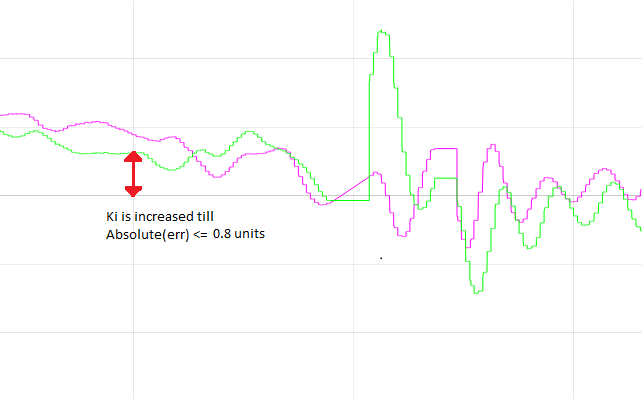
\includegraphics[width = 8cm , height= 5cm]{Autotune_iteration_1_e2.png}


\href{https://github.com/eYSIP-2018/Autotuning-of-Controller-For-Drone/blob/Amit-Kumar/Auto_Tuning.py}{Click here} to access the python program for Iteration Based Auto - Tuning\\


\subsubsection{Understanding the code }

These small snippets from the code will help in understanding it better

\begin{enumerate}
\item We subscribe to the co ordinates given by camera overhead


\hspace{0.5cm}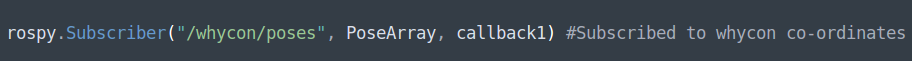
\includegraphics[width = 12cm , height= 1cm]{whycon_1.png}

\item The global variables for the x, y and z co ordinate store the float values given by the camera.


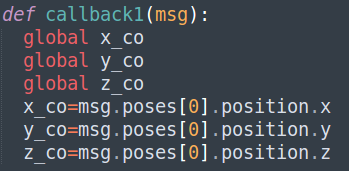
\includegraphics[width = 5cm , height= 2cm]{Callback_2.png}


\item Initialisation function asks for the input range for the PID parameters


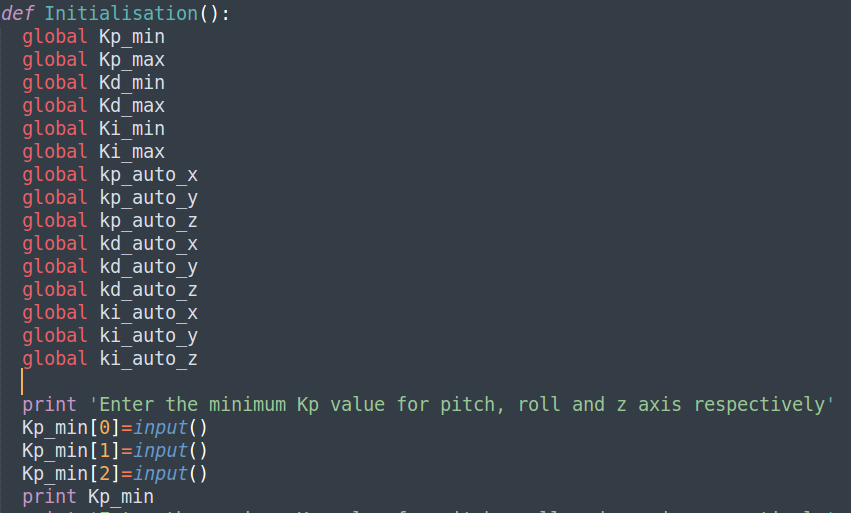
\includegraphics[width = 12cm , height= 7cm]{Initialisation_3.png}


\item A node is initialised to publish commands to drone.


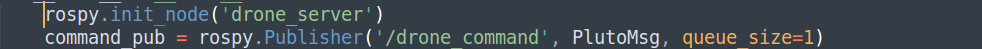
\includegraphics[width = 12cm , height= 0.7cm]{Drone_pub_5.png}

\item This part publishes the necessary values for the drone to get armed.


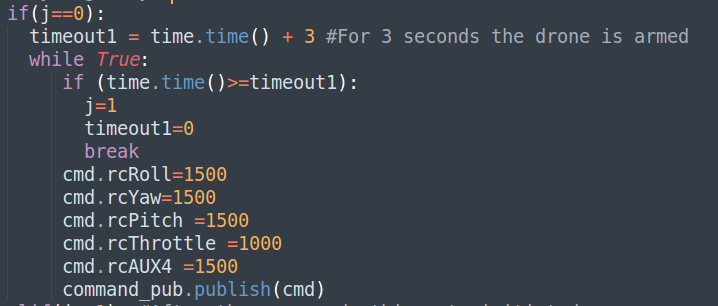
\includegraphics[width = 7cm , height= 3cm]{Arm_4.png}

\item After 3 seconds, the code enters into the auto tuning state.

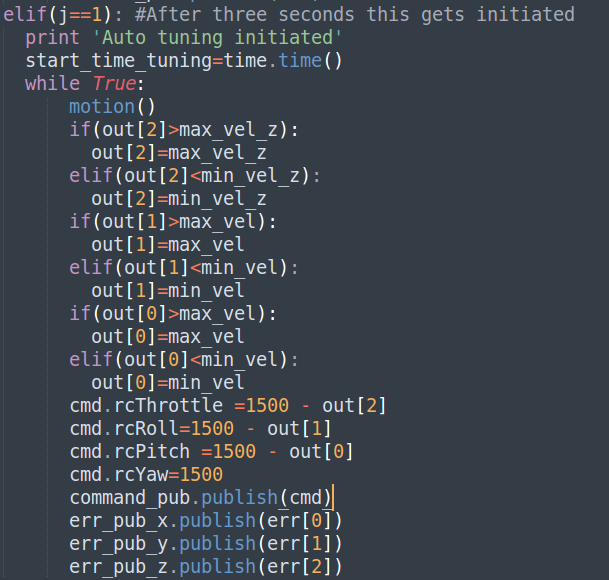
\includegraphics[width = 10cm , height= 8cm]{Auto_init_6.png}

\item The motion function helps in setting the initial values given by the user and calculating the error between the set point and the current position.

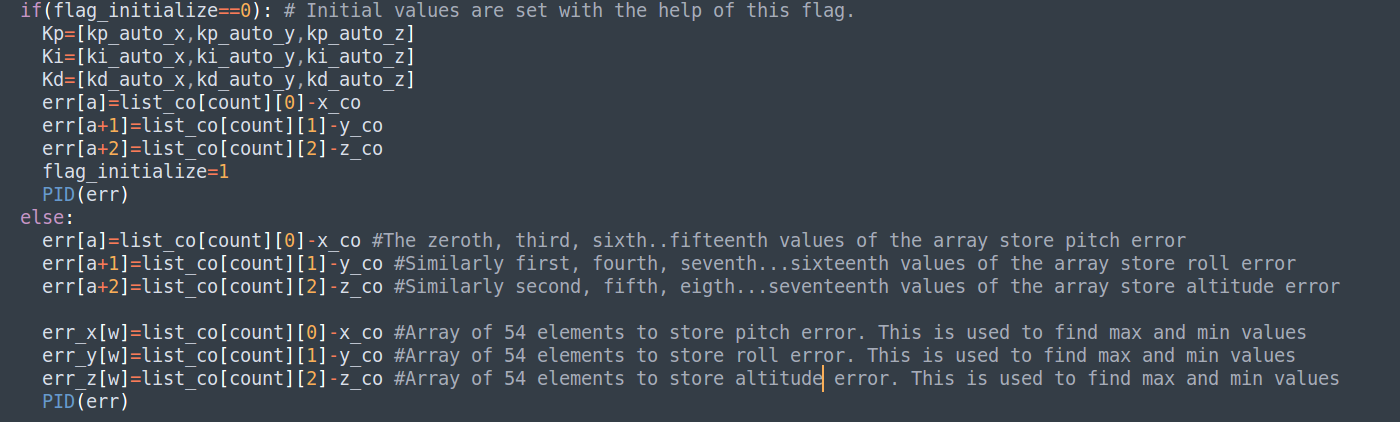
\includegraphics[width = 14cm , height= 6cm]{motion_fn_7.png}


\item The motion function calls and passes the error to PID function for calculating the PID output. A sample time of 23000 micro seconds is used. This is the time it takes for the communication to take place between drone and the code.


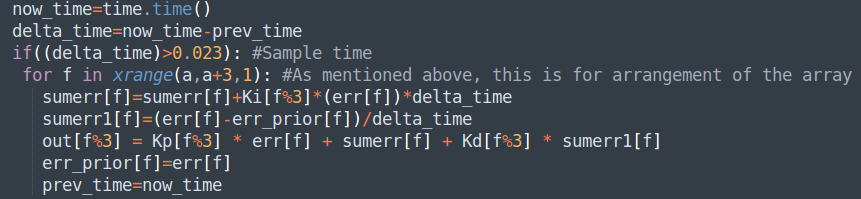
\includegraphics[width = 13cm , height= 3cm]{PID_err_8(1).png}


\item Since the co ordinates update at a frequency of 30 Hz, sampling is applied here as well. Kp tuning gets initiated.


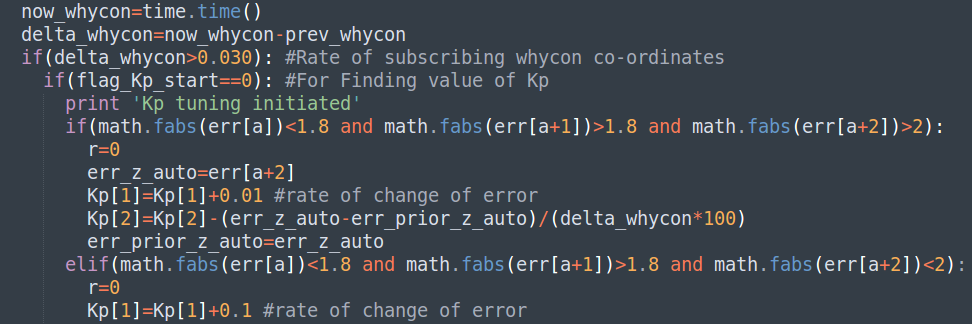
\includegraphics[width = 13cm , height= 6cm]{PID_err_8(2).png}


\item If the drone enters into an imaginary sphere of approximately 1.8 units radius, Kp tuning gets completed.


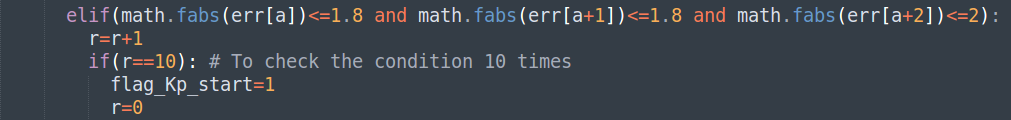
\includegraphics[width = 13cm , height= 2cm]{PID_err_8(3).png}


\item After Kp, Kd tuning gets initiated. The code continuously monitors the amplitude of the error graph and increases Kd wrt rate of change of error. If twice the amplitude is less than 1 unit for x and y axis and less than 1.6 units for the z axis (for 10 cycles) then next part of the code starts. 


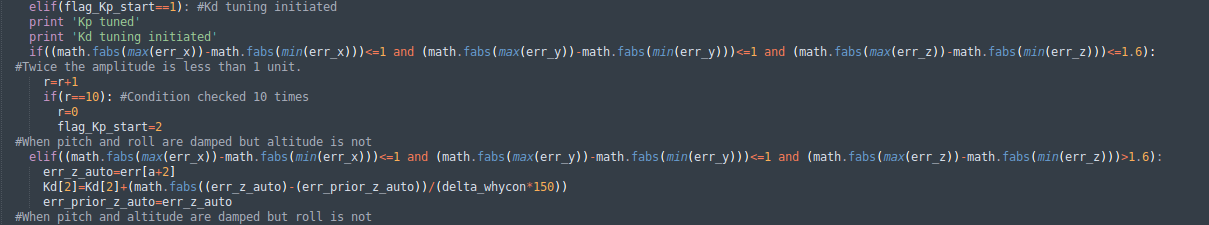
\includegraphics[width = 14cm , height= 5cm]{PID_err_8(4).png}


\item An important addition to this part is to take care of the condition where over damped case in any of the axis might arrive.
Hence if twice the amplitude is greater than 2 units in the x and y axis, Kd starts to reduce wrt rate of change of error.

Video link describing the problem and solution is mentioned in the Challenges Section.

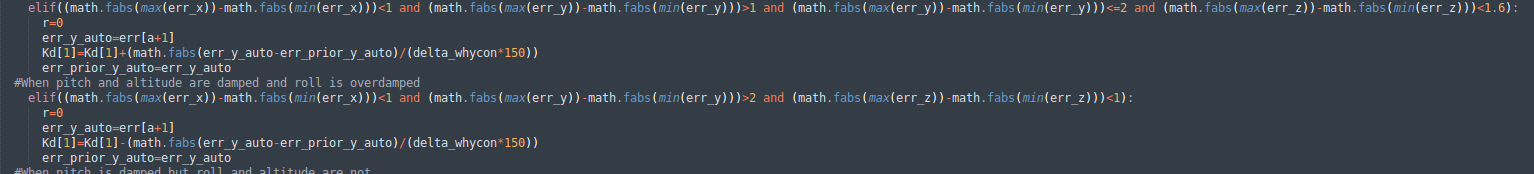
\includegraphics[width = 13.5cm , height= 3cm]{PID_err_8(5).png}


\item From here, Ki and Kd tuning goes on simultaneously. With increase in Ki to reduce the steady state error, oscillations generally occur. Hence Kd is increased to damp the oscillations. Again as discussed above the conditions take care of the problem that might arise because of the over damped condition.

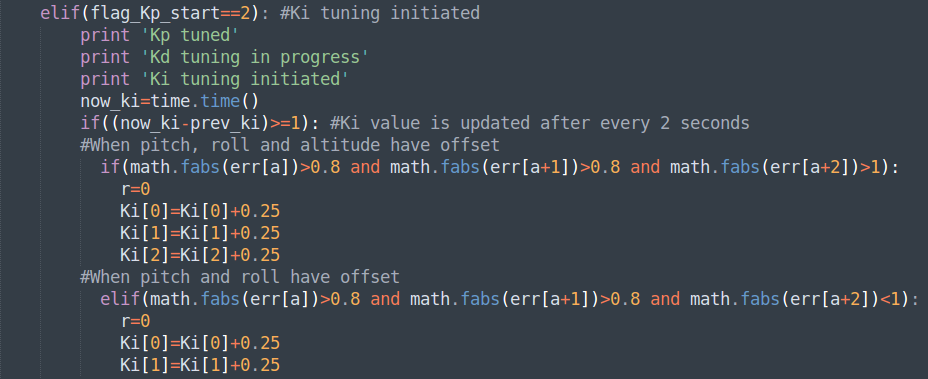
\includegraphics[width = 10cm , height= 3cm]{PID_err_8(6).png}


\item After the error is less than 0.8 units in the x and y axis and less than 1 unit in the z axis for 10 seconds, the auto tuning gets completed. From here on, Kp, Ki and Kd are constants. Way point navigation gets initiated.


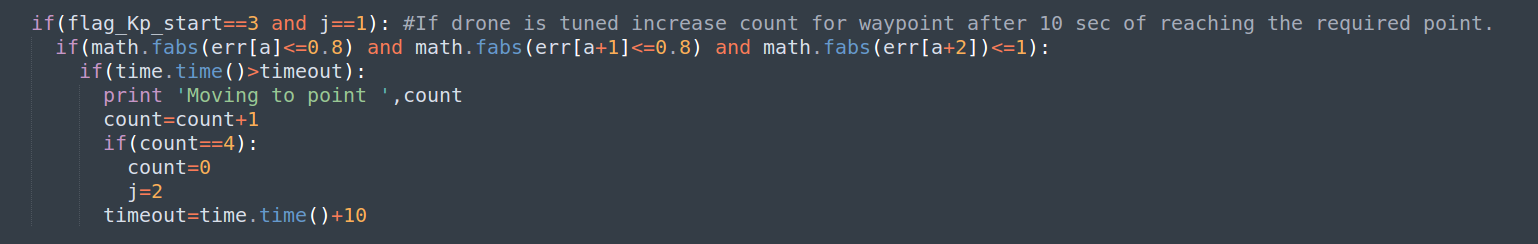
\includegraphics[width = 12cm , height= 2cm]{PID_err_8(7).png}


\item These conditions are set for all the PID parameters so that they stay in the range provided by the user.


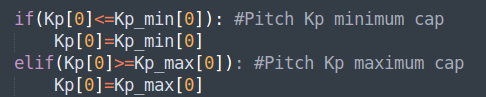
\includegraphics[width = 8cm , height= 1.5cm]{PID_err_8(8).png}


\item After way point navigation, landing gets initiated. Throttle is kept constant so that the drone slowly comes down. At the same time, PID controller keeps on working for x and y axis so that the drone lands at the same position specified by the user.


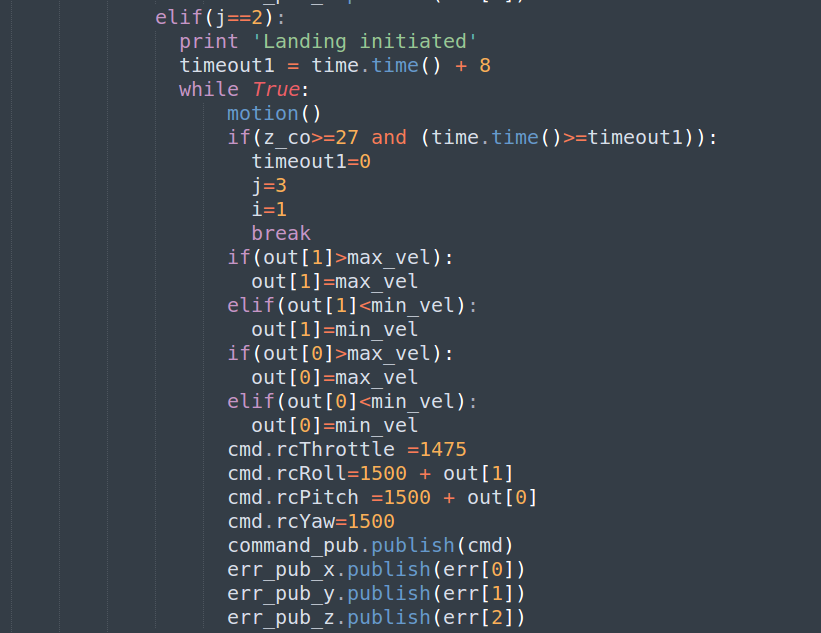
\includegraphics[width = 8cm , height= 6cm]{landing.png}


\item After landing, the drone gets disarmed.


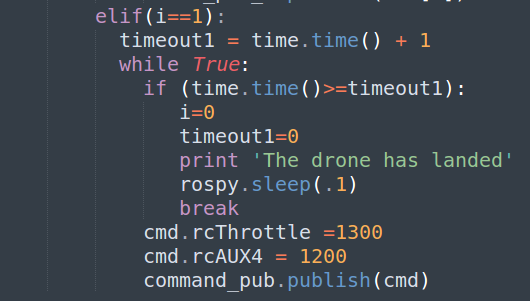
\includegraphics[width = 8cm , height= 5cm]{disarm.png}
\pagebreak
\item The error is continuously published for the graph.


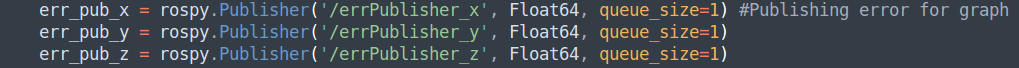
\includegraphics[width = 12cm , height= 1cm]{err_pub_9.png}

Below are couple of graphs obtained by auto tuning


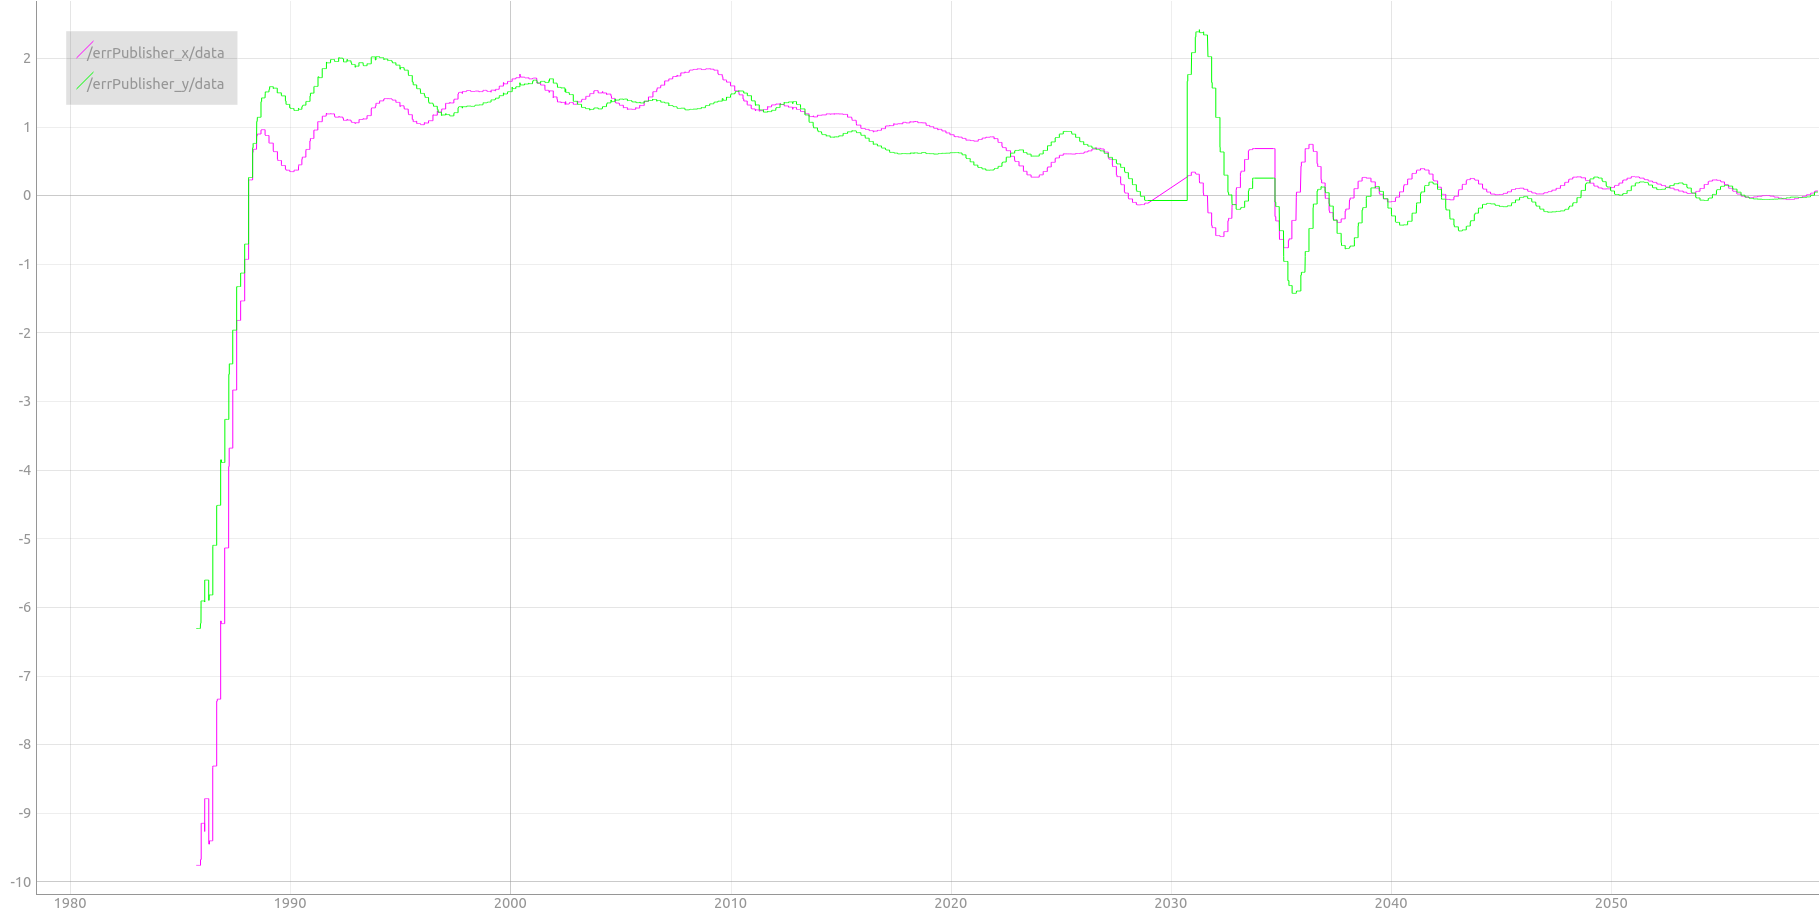
\includegraphics[width = 12cm , height= 7cm]{Autotune_iteration_1.png}


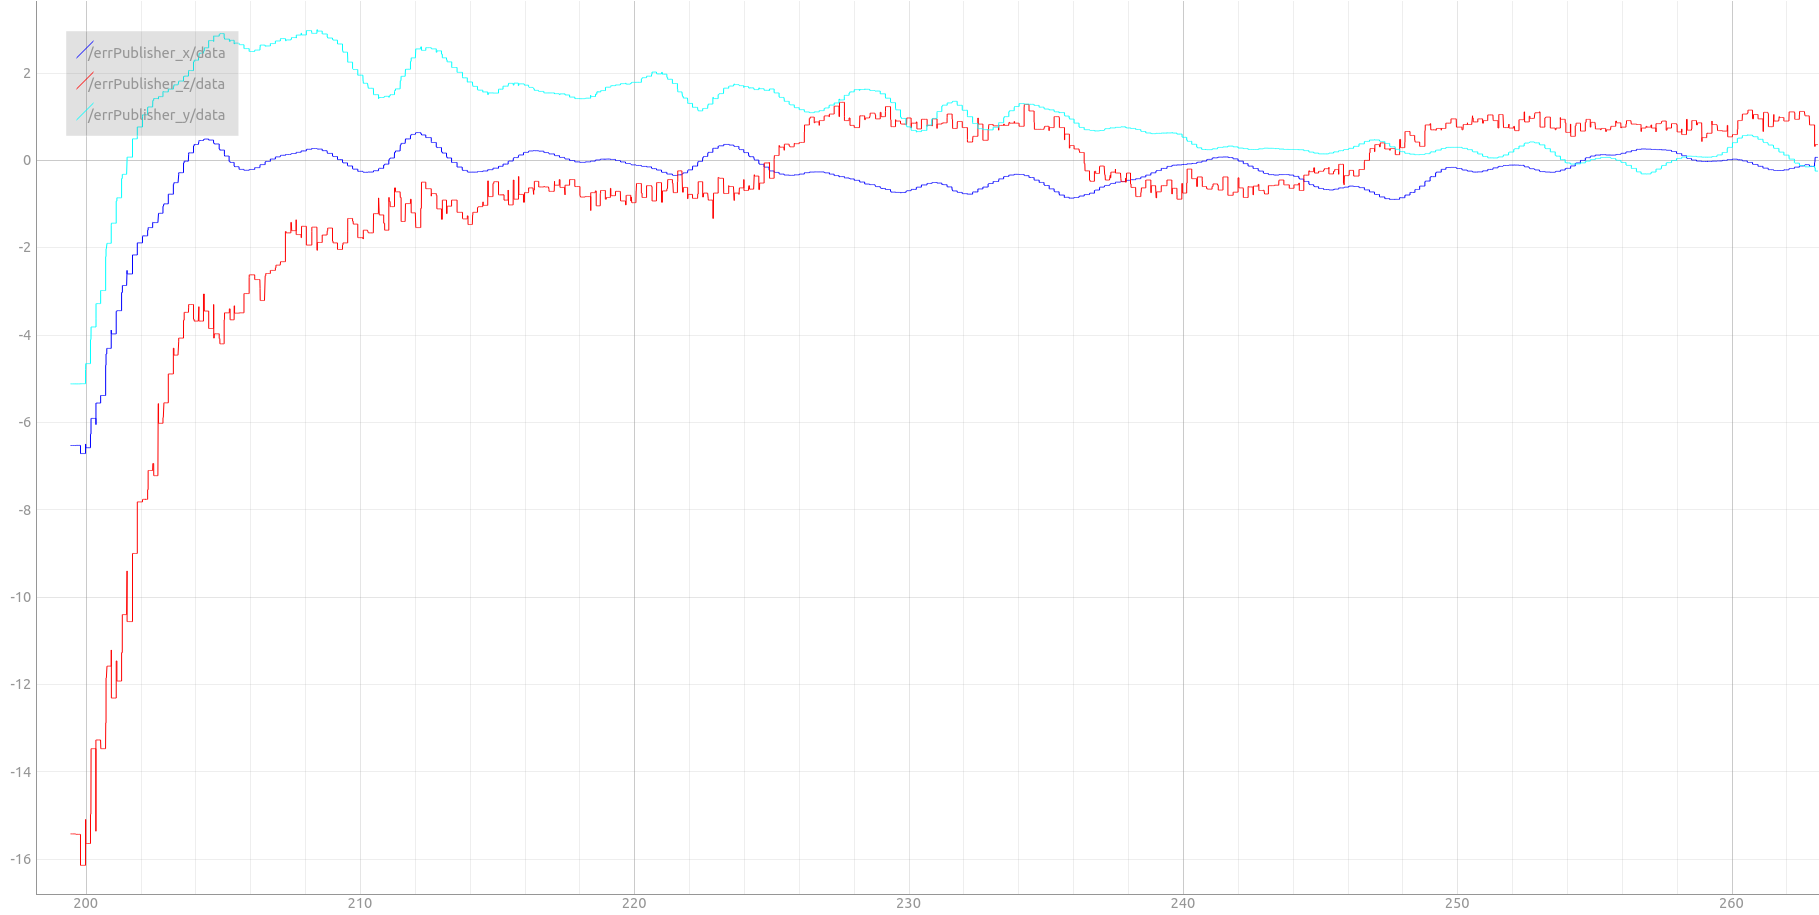
\includegraphics[width = 12cm , height= 7cm]{Autotune_iteration_2.png}

\end{enumerate}
\pagebreak
\textbf{Advantages:}\vspace{1em}
           	\begin{enumerate}
           	    \item No human monitoring or intervention required \textbf{even in a restricted frame.}
           	    \item Auto tuning takes place on the go.
           	\end{enumerate}
           	
           	
           	\textbf{Disadvantages:}
           	
           	
           	\begin{enumerate}
           	    \item On an average it takes 75 seconds for auto tuning to complete.
           	\end{enumerate}


\section{Manual Tuning versus Auto - Tuning }
One of the goals of the project was to ponder upon the advantages of auto-tuning over manual tuning.\\
The results that were obtained from auto-tuning clearly suggests that it is a more efficient way to tune the PID parameters.\\
Time taken to tune the PID parameters via auto-tuning is hardly about one minute whereas manual tuning may take an hour or sometimes even one day.\\
Manual tuning is human dependent i.e tuning depends on the person, his ability to interpret the tuning process and so on, where as auto-tuning doesn't require the human to do these mathematical stuffs.\\
As far as efficiency is concerned in terms of stability and response time, it depends on extent of tuning.\\
For example, a perfect manual tuned PID controller will have same characteristics as that of auto-tuning but a mediocre tuned PID controller will be no-match to the auto-tuning.\\
In short auto-tuning gives consistent and optimum response every time !

\pagebreak
\section{Demo}
\begin{itemize}
    \item \textbf{Auto-tuning based on Ziegler-Nichols approach}\\
    The drone is held at (0,0,20) and the code is run.\\
    The drone will first make oscillations in z axis , then in x and lastly in y axis.
    This is the auto-tuning phase.\\
    Once Kp, Ki and Kd values are obtained the way point navigation starts.
    It traverses to (-4,-4,15) , stays there for a few second then travels to (4,-4,20).After this it goes and lands on the platform at (0,0,30)
    
    \href{https://www.youtube.com/watch?v=gwrFjAuiXX0&feature=youtu.be}{Watch the demo here!}
    
    \item \textbf{Iteration Based Auto - Tuning}\\
    The drone takes off from the ground and changes the PID parameters based on the method mentioned above. After stabalisiing at (0,0,15) it goes to (-6,-4,23) and then to (-6,4,19). After completing these way points, it stabalises itself in the x and y direction and then lands on the platform.
    
    
    \href{https://youtu.be/kUO_1k9NcYQ}{Watch the demo here!}
    
    
\end{itemize}


\section{Future Work}
\begin{itemize}
    \item Currently the PID takes the input only from the whycon, to make the navigation and position holding of the drone more robust the acceleration and gyroscope inputs could be taken and be fed as other inputs to the PID.
    \item Also in the current scenario, it is observed that the whycon input of z-coordinate isn't consistent at a given point, i.e consecutive camera frames give variation in z-coordinate even if it is as the same point. This makes the PID controller confused due to which it constantly tries to stabilise the drone. Hence there is scope for improvement in this domain. 
\end{itemize}


\pagebreak
\section{Bug report and Challenges}

\subsection{Challenges faced in Iteration Based Auto Tuning Method}
\hspace{0.5cm}Video Describing over damped PID Controller
\href{https://youtu.be/r5Gr7pc5F2s}{Click Here}


Following is the graph obtained

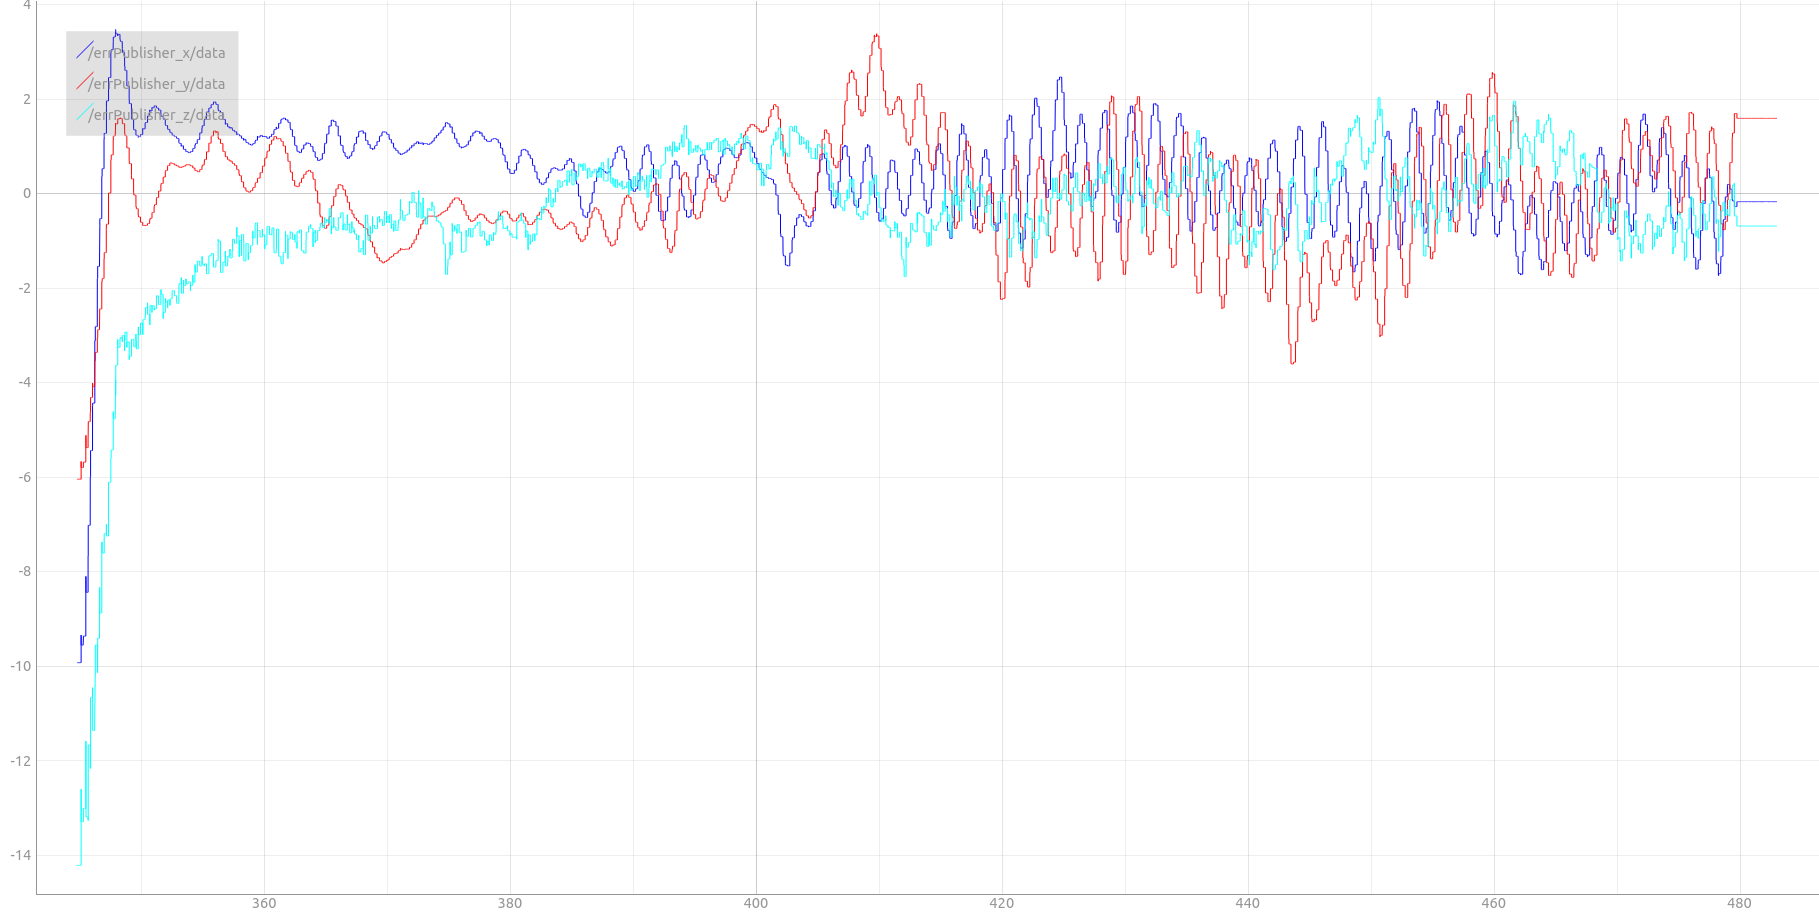
\includegraphics[width = 12cm , height= 7cm]{Overdamped.png}


Video Describing Solution for over damped PID Controller
\href{https://youtu.be/FB5wPt4SCgo}{Click Here}

Following is the graph obtained


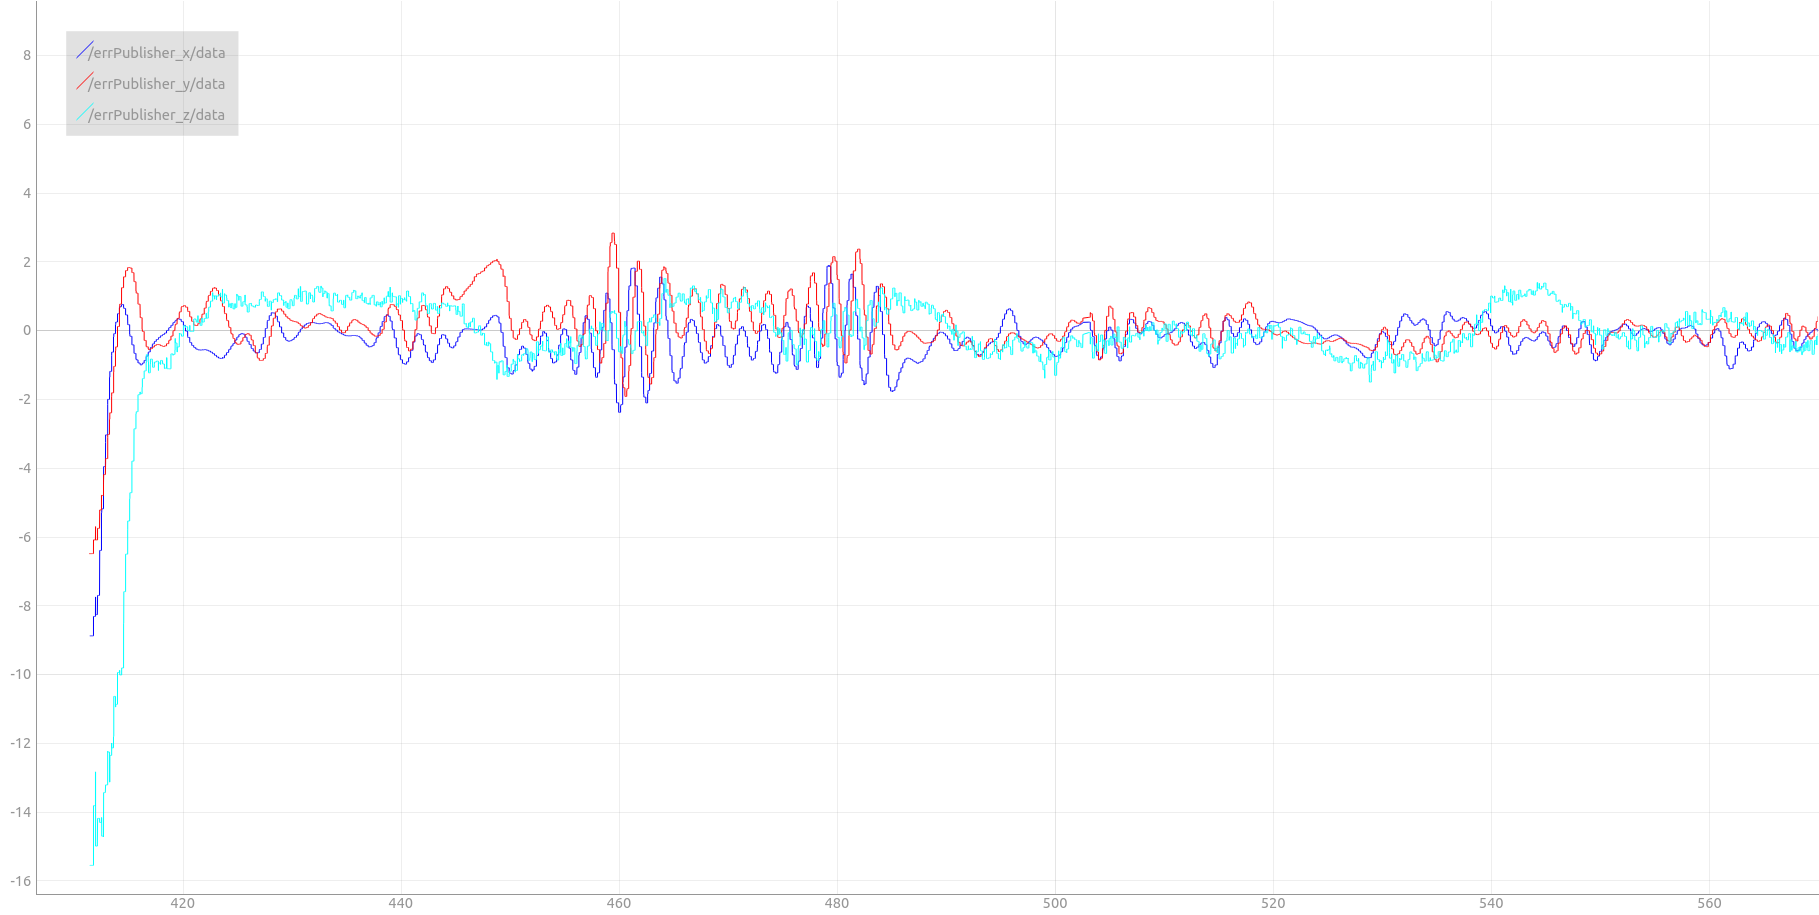
\includegraphics[width = 12cm , height= 7cm]{Overdamped_Solved.png}


Any issues in code and hardware.

Any failure or challenges faced during project
\subsection{Hardware Breakdowns}
Throughout the duration of the project there were a lot of hardware breakdowns.\\
The major failure in the hardware lied in faulty magnetometer.\\
It was observed that the magnetometer gave improper readings because of which the drone behaved inconsistently.

To check if the drone bears a proper magnetometer follow the code given in this section.\\
\href{https://github.com/eYSIP-2018/Autotuning-of-Controller-For-Drone/tree/master/magnetometer_check}{Click here to access the ROS package }
Here are a couple of snaps that depict the behaviour of a faulty and a working magnetometer\\
\subsubsection{Faulty}
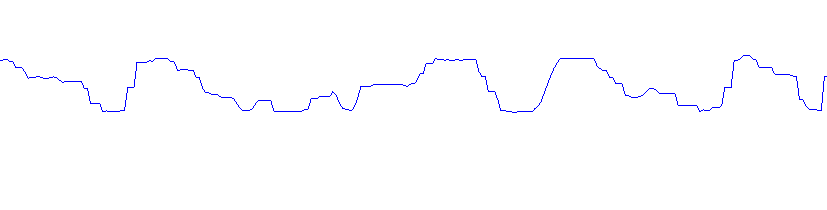
\includegraphics[width = 12cm , height= 7cm]{faulty.png}
\subsubsection{Working}
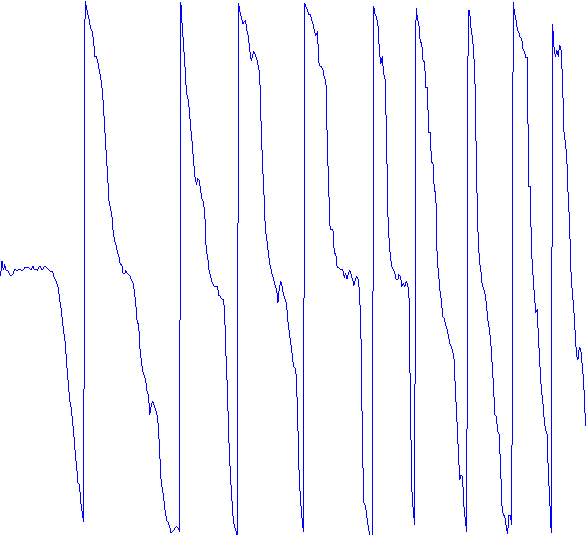
\includegraphics[width = 12cm , height= 3cm]{proper-mag.png}


%\begin{thebibliography}{li}
%\bibitem{wavelan97}
%Ad Kamerman and Leo Monteban,
%{\em WaveLAN-II: A High-Performance Wireless LAN for the Unlicensed band},
%1997.

%\end{thebibliography}

\section{References}
    \begin{enumerate}
        \item \href{http://wiki.ros.org/ROS/Tutorials}{ROS tutorials}
        \item \href{http://brettbeauregard.com/blog/2011/04/improving-the-beginners-pid-introduction/}{Improving the Beginner’s PID – Introduction}
        \item \href{https://www.youtube.com/watch?v=UR0hOmjaHp0&list=PLUMWjy5jgHK20UW0yM2    2HYEUTMJfla7Mb}{PID Control - A brief introduction}
        \item \href{https://www.youtube.com/watch?v=fusr9eTceEo}{Hardware Demo of a Digital PID Controller}
        \item \href{https://www.youtube.com/watch?v=4Y7zG48uHRo}{Controlling Self Driving Cars}
         \item \href{http://brettbeauregard.com/blog/2012/01/arduino-pid-autotune-library/}{Arduino PID Autotune Library} 
        
    \end{enumerate}

\end{document}

